\documentclass[oneside,senior,etd]{BYUPhys}

\usepackage[utf8]{inputenc}
\usepackage{rotating} 

\usepackage[english, russian]{babel}
\usepackage{amsfonts} % Пакеты для математических символов и теорем
\usepackage{amstext}
\usepackage{amssymb}
\usepackage{amsthm}
\usepackage{amsmath}
\usepackage{graphicx} % Пакеты для вставки графики
\graphicspath{ {images/} }
\usepackage{subcaption}
\usepackage{color}
\usepackage[unicode]{hyperref}
\usepackage[nottoc]{tocbibind} % Для того, чтобы список литературы отображался в оглавлении
\usepackage{algorithmic} % Для записи алгоритмов в псевдокоде
\usepackage{algorithm}
\usepackage{verbatim} % Для вставок заранее подготовленного текста в режиме as-is
\usepackage{listings}

\usepackage{commath}
\newcommand\Tau{\mathcal{T}}
\newcommand{\R}{\mathbb{R}}
\usepackage{color}
\usepackage[colorinlistoftodos, prependcaption]{todonotes}
\usepackage{multirow}
\newcommand*{\MyIndent}{\hspace*{0.2cm}}%

\Chair{Кафедра интеллектуальных информационных технологий}
\Lab{~}
\Year{2020}
  \Month{Май}
  \City{Москва}
  \AuthorText{Автор}
  \Author{Морозов Виктор Евсеевич}
  \AuthorEng{Viktor Morozov}
  \AcadGroup{620}

  \TitleTop{Методы прогнозирования потоков}
  \TitleMiddle{сложноструктурированных событий} % leave empty if you don't need it
  \TitleBottom{} % leave empty if you don't need it
  \TitleTopEng{}
  \TitleBottomEng{} % leave empty if you don't need it  
  \docname{МАГИСТЕРСКАЯ ДИССЕРТАЦИЯ}
  \Advisor{к.ф-м.н. Петровский Михаил Игоревич}
  \AdvisorDegree{}

\Abstract{}
\AbstractEng{Abstract}


%%%% DON'T change this. It is here because .sty does not support cyrillic cp properly %%%%
\University{Московский государственный университет имени М.В. Ломоносова}
\Faculty{Факультет вычислительной математики и кибернетики}
\GrText{гр.}
\AdvisorText{Научные руководители}
\AbstractText{Аннотация}

\begin{document}
\fixmargins
\makepreliminarypages

\oneandhalfspace

\tableofcontents

\section{Введение}
\label{sec:intro} \index{intro}
% \cite{theft_of_funds}.

%% Введение глобальное описание задачи (предметной области)
%% Введение: про события: сложноструктур.
%% Введение: прогнозироване: задачи регрессии / классификации
%% Актуальность (во введении) добавить: почему важно, где применяется, что может дать
%% Актуальность: в большинстве задач события имеют нерегулярную разнородную структуру: числ/катег признаки, текст етц. Хочется уметь прогнозировать вероятность наступления события / прогнозировать число событий в период времени
\subsection{События и сложноструктурированные события} \label{sect:complex_struct_event}
Задачи обработки и прогнозирования потоков событий в огромном количестве встречаются в современном мире. На практике эти задачи можно встретить при прогнозировании таких вещей как цены на бирже, автомобильный траффик, число заказов такси, количество покупок и многих других, то есть практически в любой задаче обработки данных, имеющих временн\textit{у}ю структуру. 

\textit{Поток событий} -- упорядоченный по времени набор событий, каждое из которых описывается некоторым набором признаков и имеет временн\textit{у}ю метку. 

События называются \textit{сложноструктурированными}, если они имеют сложную (нерегулярную, разнородную) структуру, т.е. эти события описываются  разнородными признаками - числовыми, категориальными, бинарными,  текстовыми. 

Сложная структура обычно возникает в том случае, когда событие описывается разнородными признаками. Умение работать с такой структурой важно в тех случаях, когда необходимо использовать максимальное количество доступной информации о событии, в том числе текстовой. Например, для прогнозирования цен на бирже было бы уместно использовать сообщения в соцсетях, новости и посты в блогах соответствующей тематики. Также, события некоторой тематики происходящие в мире в основном описываются категориальными признаками, такими как ''страна'', ''город'' и другими. Также нередки случаи, когда доступны текстовые описания для таких событий. Эффективное использование всей доступной информации может значительно улучшить качество прогнозирования.

Из определения видно, что временные промежутки между событиями не предполагаются равными.  Поскольку для применения большинства существующих методов прогнозирования и анализа временных рядов требуются одинаковые временные интервалы между событиями, нам необходимо уметь производить агрегацию признаков событий по времени. Учитывая, что значения признаков этих событий сложно агрегировать в силу их сложной структуры (особенно категориальные и текстовые признаки), возникает проблема использования накопленных данных для прогнозирования таких событий. Таким образом перед непосредственно прогнозированием возникает задача специального представления этих событий, обладающего некоторым набором свойств. В этот набор в первую очередь входят интерпретируемость и возможность агрегации по времени. Одним из подходящих методов представления является преобразование исходных значений признаков в многомерный числовой ряд, так как задачи прогнозирования временных рядов широко изучены, а сами временные ряды обладают четкой структурой.

\subsection{Задача прогнозирования} \label{sect:event_forecast}
Задачей прогнозирования в общем случае является нахождение значений  переменной отклика в какой-то момент времени в будущем в зависимости от значений объясняющих переменных в предшествующие моменты времени.

Если рассматривать задачи прогнозирования событий, то среди них можно выделить 2 основных подхода:
\begin{itemize}
    \item \textbf{Определение вероятности наступления события}
        Необходимо предсказать вероятность $p$ наступления некоторого события в течение временного промежутка в будущем. Поскольку переменная отклика в этой задаче представляет собой вероятность наступления события, то ее возможные значения находятся в диапазоне от 0 до 1. 
        
    \item \textbf{Определение количества событий, которые произойдут}
        Необходимо предсказать количество $N_e$ событий с заданными характеристиками, которые произойдут в течение некоторого временного промежутка в будущем. Переменная отклика в данном случае является счетчиком событий, то есть принимает неотрицательные значения.
\end{itemize}
\newpage
\subsection{Актуальность}
Поскольку в большинстве решаемых задач события обладают нерегулярной разнородной структурой и описываются числовыми, категориальными, бинарными и текстовыми признаками, важно уметь использовать всю доступную информацию. Возможность использования таких признаков позволит улучшить качество прогнозов, но учитывая, что события обладают сложной структурой и происходят через произвольные и неравномерные интервалы времени, использование любых признаков кроме бинарных и числовых и их агрегация затруднительны. Для того, чтобы это было возможно, необходима разработка методов представления таких сложноструктурированных событий.

Сама задача прогнозирования потоков событий в целом (включающая в себя как задачу прогнозирования вероятности, так и задачу прогнозирования количества событий) также является чрезвычайно важной, поскольку область применения такого прогнозирования крайне широкая, а умение выявлять в потоках событий скрытые зависимости находит применение во многих областях и позволяет принимать превентивные меры при правильном прогнозировании наступления событий в будущем. В качестве нескольких примеров можно привести задачи прогнозирования цен акций, предсказания выхода оборудования из строя, оценки дорожного трафика в ближайшем будущем и определения вероятности перехода пользователя по некоторой ссылке, прогнозировать количество заказов такси. Естественно, область применения не ограничена этими примерами, так как практически любую задачу предсказания чего-либо можно сформулировать в терминах задачи прогнозирования событий.

Общие подходы, решающие одновременно и задачу поиска представления сложноструктурированных событий, и задачу их прогнозирования не рассматривались в литературе, а разработка такого подхода позволит универсальным образом решать задачу прогнозирования для любых сложноструктурированных событий без необходимости создавать какие-то признаки вручную основываясь на экспертных знаниях в области решаемой задачи. % Введение
\section{Постановка задачи}
\label{sec:task_statement} \index{task_statement}

Постановка задачи:
\begin{enumerate}
    \item Исследовать и разработать интерпретируемую модель представления потоков сложноструктурированных событий, имеющих числовые, категориальные и текстовые признаки с возможностью адекватной агрегации по времени
    \item Исследовать возможность применения предложенной модели представления для прогнозирования вероятности наступления определенных событий или их количества за заданный промежуток времени
\end{enumerate}
 % Постановка задачи
\section{Обзор существующих подходов}
Цель данного обзора состоит в исследовании основных подходов к решению рассматриваемой задачи, изучении существующих моделей представления сложноструктурированных событий и методов, применяемых для прогнозирования потоков таких событий.

\subsection{Представление событий}
% (общее, теория) \\
Первым этапом исследований во всех рассмотренных работах был переход от потоков событий к временным рядам.

\subsubsection{Простые события}\label{no_struct_events}
Переход к временным рядам не составляет сложности в задачах, где у событий признаки отсутствуют и ставится задача предсказания количества событий, которые произойдут в течение некоторого временного периода. В таком случае какое-то определенное представление событий не требуется и поток событий просто преобразуется в одномерный временной ряд, где каждое значение это количество произошедших событий. Далее в этих работах авторы сразу переходят к предложениям по прогнозированию таких временных рядов.

Таким образом и поступают авторы \cite{traffic_flow_forecasting}, при решении задачи прогнозирования автомобильного траффика. Хотя в этой статье и описывается подход прогнозирования траффика с использованием разнородных источников данных, эти данные представляют из себя одномерные временные ряды, что избавляет авторов от задачи поиска подходящей модели представления событий. В работе \cite{modeling_patterns_with_DNN} и \cite{predictive_monitoring_LSTM} авторы акцентируют внимание на решении задачи прогнозирования и поиска паттернов во временных рядах, опять же, без необходимости реализации какого-то сложного представления данных.

\subsubsection{События с относительно простой структурой} \label{simple_struct_events}
В задачах, где событие описывается какими-то признаками, подходы к представлению таких событий могут быть сильно различаться от задачи к задаче, но многие из них объединяет общий подход, состоящий в формировании формулы для вычисления значений признаков для событий экспертами, следовательно эти признаки специфичны для какой-то отдельно взятой области, и их не получится легко перенести на задачу из другой области.

Так, например, в работе \cite{twitter_predicting} событиями являются посты в сети Twitter (твиты) и для этих событий создаются различные ориентированные на их структуру (текст, возможно ссылки, хэштеги) признаки, а так же признаки, специфичные для задачи, такие как исторические изменения популярности каких-то тем, соответствующих твиту. 
В работе \cite{triplet_event_forecasting}, каждое событие представляет собой триплет вида (объект -- URL, субъект -- пользователь, временная метка -- время клика), а в качестве признаков для прогнозирования используются взаимодействия объектов и субъектов на протяжении какого-то временного интервала.

В работе \cite{uber_mulitvar_forecasting} описание событий является многомерным временным рядом, такое представление является более сложным, чем представление, описанное в \ref{no_struct_events}, но оно так же поддерживает возможность агрегации по временным периодам (например, усреднением) и не требует какой-то предобработки признаков событий.

\subsubsection{События с разнородными признаками}
В задачах, где события описываются одним и тем же набором числовых, категориальных, бинарных и, возможно, текстовых признаков, необходимо использовать какое-то представление для событий.

С бинарными признаками в общем случае можно работать как с числовыми, а категориальные признаки приводятся к бинарным с помощью подхода One-Hot Encoding или обрабатываются любым другим способом (value encoding/label encoding/target encoding)
С текстовыми описаниями все сложнее, но в общем виде все равно требуется получить какое-то числовое (векторное) представление текста. Для решения этой задачи можно применять как классические подходы к тематическому моделированию, (TF-IDF, LDA), так и более современные подходы, в том числе использование word2vec или LSTM для получения эбмеддингов (векторных представлений) слов, предложений или целых документов.
После обработки, все эти признаки можно объединить в новый вектор признаков, которые будут исключительно числовыми, и дальше работать с новыми признаками как описано в \ref{simple_struct_events}

В случае со сложноструктурированными событиями иногда часть признаков не используется, так в работе \cite{comparison_coronary_heart_disease} из 16 разнородных медицинских признаков были выделены 10 числовых признаков и прогнозирование заболеваний сердца производилось только с их использованием. Такой подход имеет право на существование, но не использует всю доступную информацию.

В работе \cite{struct_unstruct_prediction} используются табличные данные, которые по своей природе очень просто привести к временным рядам, вместе с ними используются неструктурированные текстовые данные, полученные из открытых источников, затем производят многоклассовую классификацию каждого документа, где классы это набор заранее определенных рубрик. После классификации авторы получают из неструктурированных текстовых данных многомерный числовой ряд (вероятности принадлежности текстового документа к конкретной рубрике), размерность которого соответствует количеству различных рубрик. В итоге авторы используют этот временной ряд наряду со структурированными данными для прогнозирования.

\subsection{Прогнозирование событий}
% (общее, теория) \\
Задачей прогнозирования событий в общем случае является нахождение значений целевой переменной отклика в какой-то момент времени в будущем. Чаще всего рассматривается одна из подзадач: определение количества событий, которые произойдут, или определение вероятности того, что событие произойдет.

%%% REGRESSION
\subsubsection{Задача прогнозирования количества событий}
Особенностью задачи прогнозирования количества событий является то, что целевая переменная (отклик) может принимать произвольные (обычно неотрицательные) значения. В качестве примера можно привести задачу прогнозирования количества продаж товара в течении следующей недели, количества заказов такси в течение следующих суток и многие другие задачи, встречающиеся в реальной жизни. Такие задачи прогнозирования количества событий мы будем называть задачами регрессии.

Авторы многих работ предлагают решения, основанные на применении глубоких нейронных сетей, в частности авторы \cite{traffic_flow_forecasting} предлагают использовать связку CNN и RNN для прогнозирования дорожного траффика на каком-то определенном участке дороги в каком-то определенном временном интервале, то есть решается задача регрессии.

В работе \cite{modeling_patterns_with_DNN} авторы также используют сочетание CNN и RNN для прогнозирования многомерных временных рядов, т.е. для решения задачи регрессии значений временного ряда. Особенность сочетания CNN и RNN в том, что CNN позволяет моделировать локальные зависимости на коротких промежутках времени, а RNN позволяет моделировать долгосрочные временные зависимости.

Авторы \cite{predictive_monitoring_LSTM} используют LSTM для задачи прогнозирования логов, например, для предсказывания времени, которое потребуется на завершение некоторой задачи.

В работе \cite{uber_mulitvar_forecasting} решается чистая задача регрессии: авторы с помощью рекуррентных нейронных сетей прогнозируют количество вызовов такси в заданном временном интервале. 

Подход авторов работы \cite{triplet_event_forecasting} отличается от перечисленных выше. В этой работе авторы, решая общую задачу поиска паттернов в переходах пользователей по различным URL, в частности рассматривая задачу прогнозирования объема траффика от конкретного пользователя (задачу регрессии). Для ее решения применяются авторегрессионные методы.

%%% CLASSIFICATION
\subsubsection{Задача прогнозировании вероятности события}
Определение вероятности наступления события -- задача, в которой значение целевой переменной (отклика) характеризует вероятность наступления события. Чаще всего в таких задачах отклик принимает значения в диапазоне от 0 до 1. Задачи прогнозирования такого рода мы будем называть задачами классификации.

Задачи классификации охватывают широкий спектр проблем и включают в себя задачу бинарной классификации (напр. произойдет или нет определенное событие в будущем), задачу многоклассовой классификации (напр. какое событие из нескольких возможных с наибольшей вероятностью произойдет в будущем) и задачу поиска аномалий (напр. определение паттерна, которые предшествует некоторым аномальным событиям).

Авторы \cite{struct_unstruct_prediction} решают задачу классификации, прогнозируя направление движения цены акций (вверх или вниз) и используют для этого нейронные сети с архитектурой LSTM. В качестве признаков используются как структурированные исторические данные из открытых источников, так и неструктурированные текстовые данные, обработанные специальным образом.

В работе \cite{twitter_predicting} описан следующий подход -- авторы на основании экспертных знаний формируют признаки, и используя значения этих признаков и некоторых исторических данных обучают модель классификации для прогнозируют тренда популярности определенного события. Таким образом эта работа описывает задачу многоклассовой классификации с классами "популярность вырастет", "останется на том же уровне" и 3 класса, описывающих различные по силе падения популярности.

Работа \cite{comparison_coronary_heart_disease} напрямую не описывает задачу прогнозирования событий, в этой работе рассматривается вероятность того, что событие произойдет когда-либо в будущем, и поскольку четкой авторы не используют какую-то временн\textit{у}ю структуру для описания признаков или событий, то эта задача сводится к задаче бинарной классификации и уже для этой задачи авторы сравнивают различные существующие методы классификации.

Отдельно стоит рассматривать задачу прогнозирования экстремально редких событий. Поскольку в такой задаче набор данных имеет ярко выраженный дисбаланс классов, авторы в большинстве случаев переходят от решения задачи прогнозирования к задаче поиска аномалий, таким образом они не предсказывают события, но определяют характерные паттерны, предшествующие этим редким событиям.

Для решения таких задач в качестве стандартных средств часто используются одноклассовые классификаторы, например в работе \cite{anomaly_detection_oneclass} авторы с помощью обучают одноклассовый классификатор на показаниях с датчиков станка и выявляют паттерны, предшествующие выходу оборудования из строя.

Авторы \cite{anomaly_detection_ae} предлагают использовать более продвинутые средства -- автокодировщики -- для решения задачи прогнозирования выхода оборудования из строя. В этой работе авторы высказывают предположение, что если автокодировщик, обученный на наборе показаний датчиков в случае штатной работы оборудования показывает большую ошибку в задаче кодирования и последующего декодирования показаний датчиков, то такие показания можно считать аномальными.

\subsection{Выводы из обзора}
Было проведено исследование основных подходов к двум этапам решения рассматриваемой задачи, изучены существующие методы представления как сложноструктурированных, так и достаточно простых объектов и методы, применяемые для прогнозирования временных рядов. По результатам исследования сделаны следующие выводы:
\begin{itemize}
    \item для представления событий чаще всего используются признаки: описанные экспертами и соответствующие тематике задачи (\cite{twitter_predicting}), в некоторых работах ищется автоматическое представление, но только для текстовых описаний (\cite{struct_unstruct_prediction}).
    \item для прогнозирования событий чаще всего используются нейронные сети (CNN + RNN: \cite{traffic_flow_forecasting}, \cite{modeling_patterns_with_DNN}; LSTM: \cite{uber_mulitvar_forecasting}, \cite{predictive_monitoring_LSTM}, \cite{struct_unstruct_prediction});
    \item для экстремально редких событий можно использовать подход поиска аномалий, т.к. остальные методы прогнозирования показывают себя плохо при сильном дисбалансе классов.
    \item не существует какого-то общего подхода, объединяющего одновременно поиск представления сложноструктурированных событий, и прогнозирование этих событий.
\end{itemize}

Основным направлением дальнейшей работы будет являться как исследование и разработка представления сложноструктурированных событий в виде исключительно числовых признаков, так и прогнозирование этих событий.
 % Обзор существующих решений
\section{Исследование и построение решения задачи}
\label{sec:research_and_solving} \index{research_and_solving}
\subsection{Описание предложенного решения задачи}
В этом разделе будет описаны методы построения представления сложноструктурированных событий, рассмотрена интерпретируемость каждого из представлений, и показано, какие методы можно использовать для решения  непосредственно задачи прогнозирования.

Схема предложенного подхода к решению поставленной задачи показана на Рис. \ref{fig:framework_structure}, далее в этой секции будут детально описаны все компоненты предложенного подхода.

\begin{figure}
    \centering
    \includegraphics[width=\linewidth]{images/framework_scheme.png}
    \caption{Структура предложенного подхода}
    \label{fig:framework_structure}
\end{figure}

\subsubsection{Построение представления событий}
\label{subsub:repr}
% PCA
% NMF Неотрицательная факторизация матрицы
% AE Нейросетевой автокодировщик
При построении представления сложноструктурированных событий и с учетом их временной неравномерности,
мы требуем от такого представления возможность агрегации по времени. Также для неявного (скрытого) представления событий хотелось бы иметь возможность его интерпретации, чтобы можно было производить какой-то анализ как самого представления, так и использующих его моделей.

Перед переходом к построению представления, опишем предлагаемые методы обработки различных типов признаков.
Числовые и бинарные признаки не предобрабатывались, категориальные признаки переводились в бинарные с помощью унитарного кодирования (one-hot encoding). Для категориальных признаков также можно использовать любой метод перевода их в бинарные/числовые признаки: кодирование уникальными значениями и другие.
Текстовые описания можно преобразовать в числовые вектора одним из многих способов: латентным размещение Дирихле (LDA), кодированием tf-idf или нейросетевыми моделями (word2vec, doc2vec, скрытое представление с помощью LSTM). В этой работе я использовал латентное размещение Дирихле для предобработки текстовых данных. После такой обработки все признаки становятся либо числовыми, либо бинарными.

Несмотря на то, что числовые и бинарные признаки обладают возможностью агрегации по времени, велика вероятность того, что они избыточны, а значит можно найти такое представление, которое переведет исходные признаки в пространство меньшей размерности и будет более уместно для использования в задаче прогнозирования. 

В качестве базового подхода были рассмотрены такие методы понижения размерности как Метод главных компонент (PCA \cite{pca_orig}), Неотрицательная факторизация матриц (NMF \cite{nmf_orig}). В этой работе было решено остановиться на более тщательном исследовании применимости неотрицательной факторизации матриц. 

Общая идея факторизации матрицы заключается в следующем: 
Пусть $n$ -- количество событий, $d$ -- размерность вектора признаков каждого события. Обозначим исходную матрицу описывающую события как $V$, $V \in \mathbf{R}^{n \times d}$. Задача факторизация матрицы $V$ заключается в нахождении матриц $W \in \mathbf{R}^{n \times k}, H \in \mathbf{R}^{k \times d}$, $k \ll d$ таких, что эти матрицы $W, H$ минимизируют $||V - W \cdot H||$. Из такого разложения видно, что матрица $H$ показывает соотношение между исходными $n$ признаками и новыми $k$ признаками. Эти новые $k$ признаков мы будем в дальнейшем называть тематиками или скрытыми (латентными) признаками. Также будем называть матрицу $W$ матрицей \textit{событий-тематик}, а матрицу $H$ матрицей \textit{тематик-признаков}. Схема работы этого метода приведена на Рис. \ref{fig:nmf_scheme}.

\begin{figure}
\centering
  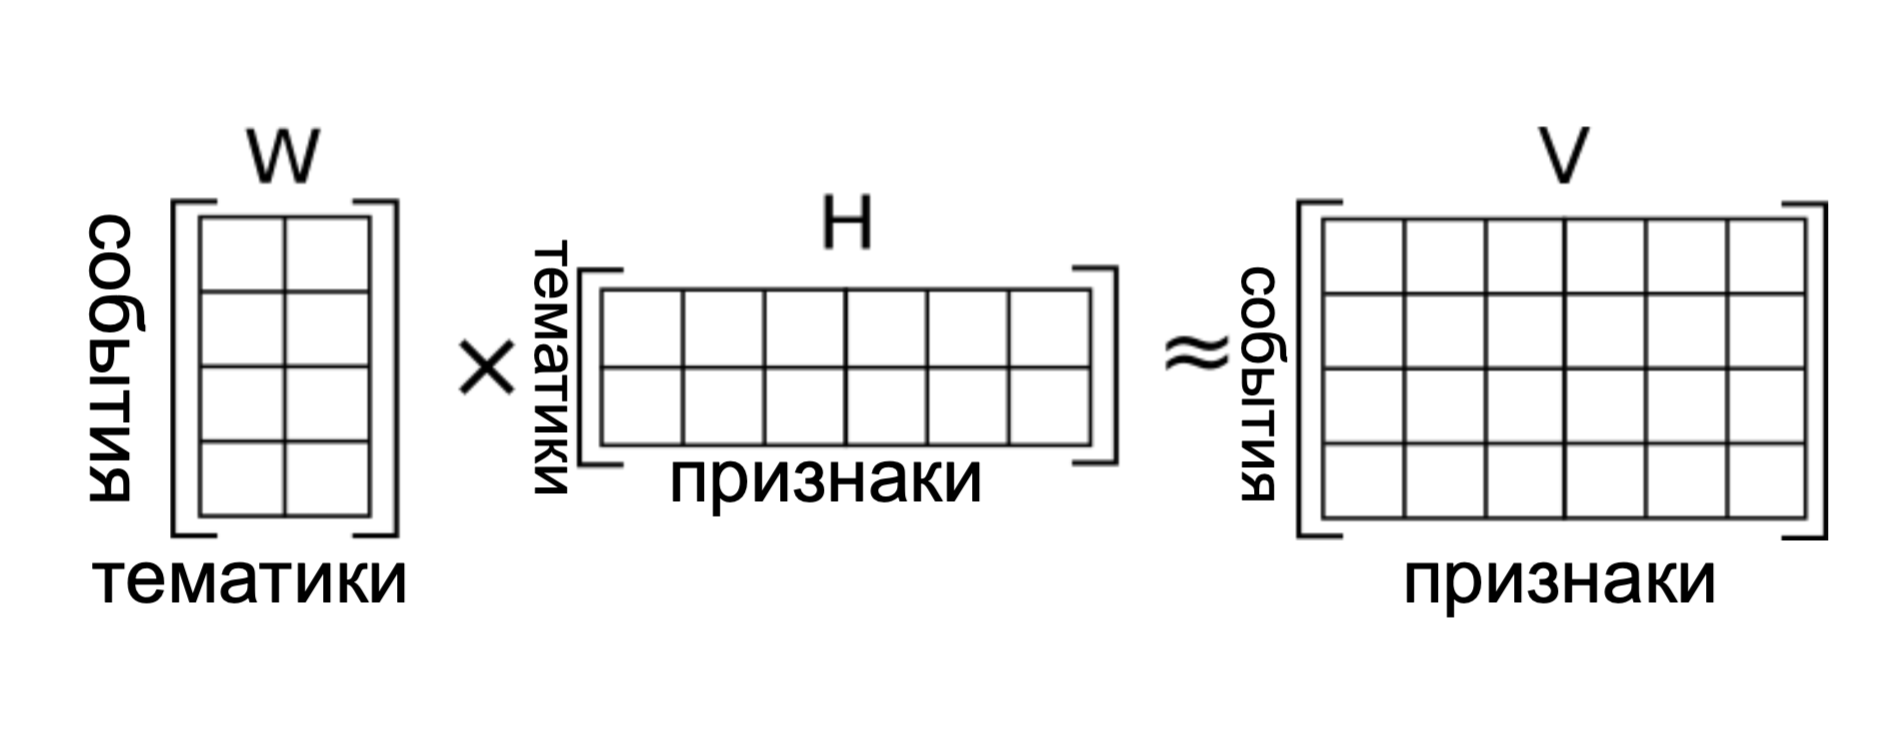
\includegraphics[width=.9\linewidth]{images/nmf_scheme.png}
  \caption{Схематическое изображение работы алгоритма NMF}
  \label{fig:nmf_scheme}
\end{figure}

При использовании неотрицательной факторизации матрицы, тематики представляют из себя линейные комбинации исходных признаков с неотрицательными весами, что делает интерпретируемость этих тематик тривиальной задачей.

Процесс факторизации является итеративным, в начале матрицы $W, H$ инициализируются неотрицательными значениями, затем они поочередно обновляются следующим образом:
$$H^{n+1}_{[i,j]} = H^n_{[i,j]} \frac{((W_n)^TV)_{[i,j]}}{((W^n)^TW^nH^n)_{i,j]}}$$
$$W^{n+1}_{[i,j]} = W^n_{[i,j]} \frac{(V(H^{n+1})^T)_{[i,j]}}{(W^nH^{n+1}(H^{n+1})^T)_{[i,j]}}$$

После того, как процесс сойдется, мы получаем матрицы $W,H$.

В качестве более продвинутого метода построения представления событий будет рассмотрен глубокий нейросетевой автокодировщик (далее -- просто автокодировщик) \cite{ae_orig}. 
Автокодировщик это специальная архитектура искусственных нейронных сетей, позволяющая применять обучение без учителя при использовании метода обратного распространения ошибки.

Простейшая архитектура автокодировщика — сеть прямого распространения, схожая с многослойным перцептроном и содержащая блок слоев для перевода входного вектора в скрытый код (кодировщик) и блок слоев для перевода скрытого кода в выходной вектор (декодировщик). В отличие от стандартных нейросетевых архитектур, выходной слой автокодировщика содержит столько же нейронов, сколько и входной слой, а задачей всей сети является перевод входного вектора в код меньшей размерности (кодировщик) и дальнейшее восстановление вектора из его кода с минимизацией ошибки восстановления (декодировщик). Пример архитектуры однослойного автокодировщика представлен на Рис. \ref{fig:ae_arch}.
\begin{figure}
\centering
  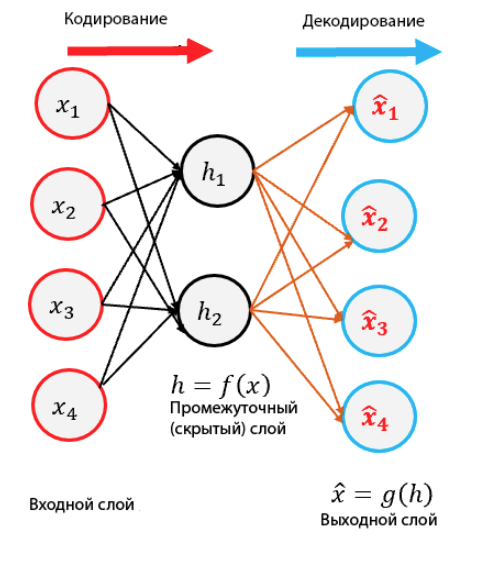
\includegraphics[width=.5\linewidth]{ae_arch_ru.png}
  \caption{Пример архитектуры простого автокодировщика}
  \label{fig:ae_arch}
\end{figure}

Более формально, автокодировщик нелинейно преобразует входной вектор $x \in \mathbf{R}^d$ в $z \in \mathbf{R}^k$, а затем производит реконструкцию вектора $x$ используя $z$. В результате реконструкции получается вектор $x' \in \mathbf{R}^d$, и задача автокодировщика -- минимизировать ошибку восстановления $L(x,x')$ (например $L(x,x')=||x - x'||$).

После обучения модели с такой архитектурой, можно использовать только ее первую часть (кодировщик) для получения $z^*$ их произвольного входного вектора $x^*$ и использовать этот код $z^*$ как скрытое представление события. В таком случае скрытыми тематиками будем называть элементы вектора $z^*$.
Так как преобразования кодировщика нелинейны, интерпретация скрытого кода затруднительна, эта проблема будет рассмотрена отдельно в следующем разделе.

% Auxiliary features
В процессе исследования решения задачи, было решено добавить два дополнительных признака для выделения более явной регрессионной компоненты. Для каждого агрегационного периода вычислялось:
\begin{enumerate}
   \item $N_{all}$, общее количество событий, входящих в этот период
   \item $N_{target}$, количество целевых событий, входящих в этот период
\end{enumerate}

Эти признаки можно было бы назвать ''экспертными'' или ''созданными вручную'', но они не умаляют общности подхода, так как применимы для задачи прогнозирования событий в целом.

% Recon features
Также вместе с признаками, полученными с помощью автокодировщика было предложено использовать в качестве дополнительного признака ошибку восстановления автокодировщика (т.е. признак, показывающий, насколько восстановленный автокодировщиком вектор признаков отличается от исходного вектора признаков):

$recon\_err = x' - x$, следуя нотации введенной ранее.

Мотивация добавления подобного признака следует из области выявления аномалий \cite{anomaly_detection_ae} и заключается в следующем: если исходный вектор признаков сильно отличается от восстановленного вектора признаков (большая ошибка восстановления), то есть основания полагать, что этот вектор является в некотором смысле аномальным и модель с помощью значения такого признака сможет учитывать аномальность конкретного события.

\subsubsection{Интерпретируемость представления}
\label{subsub:interp}
Как было сказано выше, важной характеристикой скрытого представления событий является его интерпретируемость. Если у представления такое свойство есть, то становится возможным анализ полученных тематик, а так же анализ результатов прогнозирования и их более глубокое понимание.

По своей природе скрытые признаки, выделенные неотрицательной факторизацией матриц и методом главных компонент интерпретируемы, поскольку эти скрытые признаки представляют собой линейные комбинации исходных признаков. В случае неотрицательной факторизацией матриц, если рассмотреть вышеупомянутую матрицу \textit{тематик-признаков}, можно увидеть, что каждая тематика описывается набором неотрицательных весов, соответствующих оригинальным признакам. Чем больше вес у некоторого признака, тем более сильный вклад этот признак вносит в данную тематику. 

Пример того, как можно описать одну из тематик, выделенных NMF, можно увидеть на Рис. \ref{fig:nmf_topic}. На этом рисунке изображены 9 исходных признаков с наибольшими весами, т.е. вносящих максимальный вклад в тематику. Для более полного понимания стоит заметить, что используемый набор данных содержит описания событий из реального мира -- террористических актов (подробное описание в \ref{sec:experiments}). Как можно увидеть из рисунка, наибольший вклад в тематику 2 вносят признаки weaptype1\_firearms и attacktype1\_arm\_aslt. В нашем случае это бинарные признаки, появившиеся после разложения категориальных признаков weaptype1 и attacktype1 с помощью унитарного кодирования. Значение признака weaptype1\_firearms равное 1 показывает, что было использовано огнестрельное оружие, а значение attacktype1\_arm\_aslt равное 1 показывает, что тип атаки -- вооруженное нападение. Таким образом, зная специфику данных, можно понять, что тематика 2 в основном соответствует вооруженным нападениям с применением огнестрельного оружия, такое описание и является интерпретацией тематики. 

\begin{figure}
  \centering
  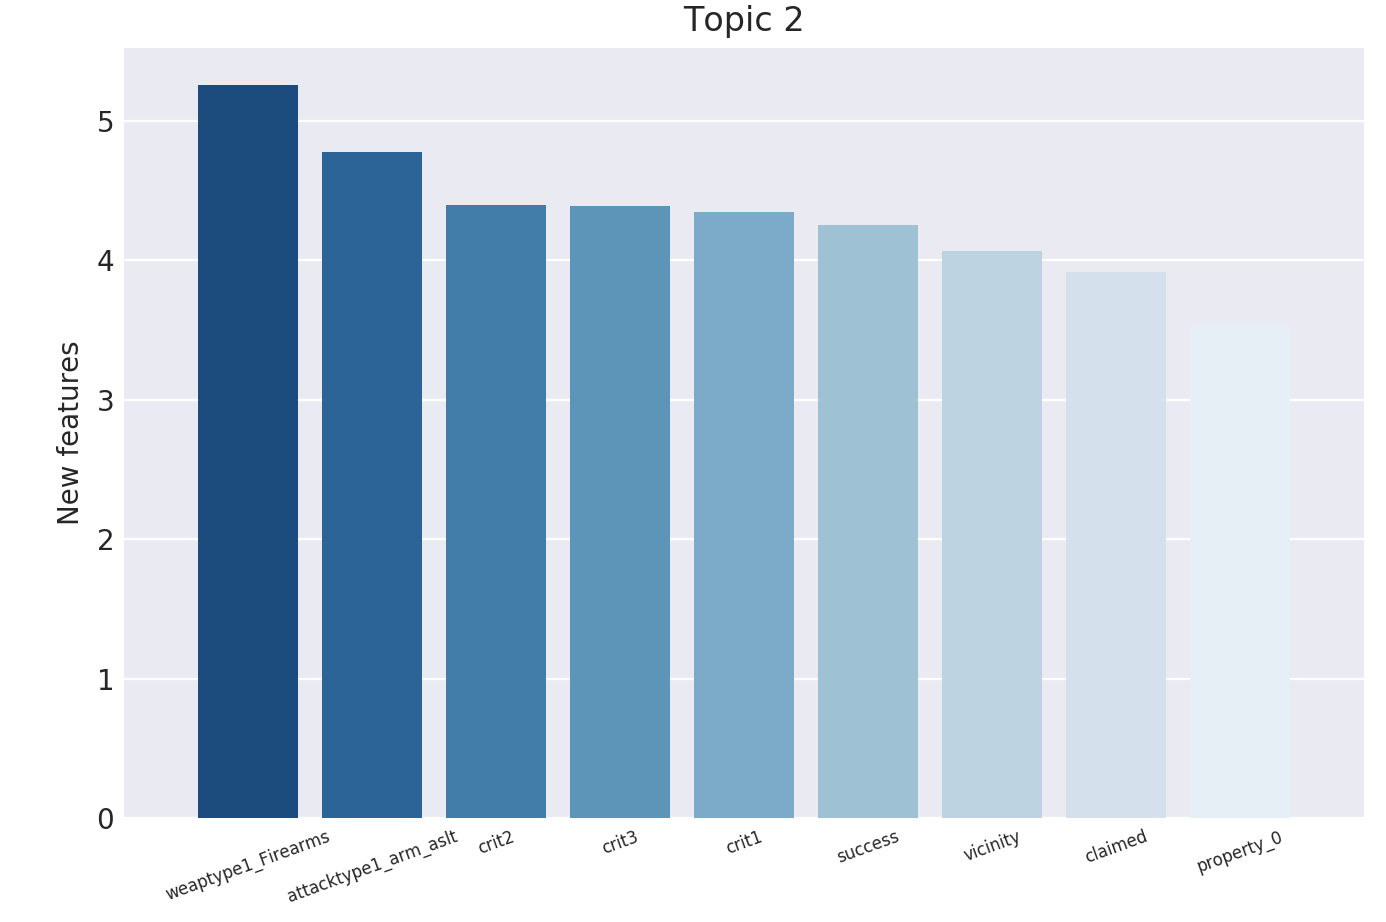
\includegraphics[width=.8\linewidth]{nmftopic.png}
  \caption{Пример интерпретации тематики, выделенной с помощью неотрицательной факторизации матриц}
  \label{fig:nmf_topic}
\end{figure}

В случае, когда преобразование исходного пространства признаков более сложное и нелинейное, необходимы другие методы интерпретации.
В данной работе предлагается метод, основанный на текстовых описаниях, доступных хотя бы для части событий.

\textit{Входными данными} для алгоритма является набор событий с текстовыми описаниям и соответствующие значения скрытых тематик для каждого из событий. Более формально, на вход подаются матрица значений скрытых тематик для событий  $T = \{t_{i,j}\}, \in \mathbf{R}^{k \times n}$ и текстовые описания событий $\{d'_j\}$.

\textit{Результатом} работы алгоритма является набор из $K$ ключевых слов для каждой из скрытых тематик, являющийся текстовым описанием этой тематики. Ниже приведено текстовое описание алгоритма, формально описание предоставлено в блоке Алг. \ref{alg:kw_interp}.

Первый шаг получения интерпретации тематик это извлечь все доступные текстовые описания, предобработать их стандартными методами обработки текстовых данных (привести к нижнему регистру, убрать пунктуацию и стоп-слова, нормализовать формы слов) и выделить все различные слова. Далее составим \textit{словарь ключевых слов} $W$ из полученного набора различных слов и обозначим размер этого словаря как $|W|$.

Затем выберем из всего множества событий те, у которых есть текстовые описания, и каждому событию сопоставим $|W|$ бинарных признаков, показывающих вхождение или отсутствие каждого слова из $W$ в текстовом описании этого события.

После составления таких признаков необходимо найти значение $v_{i,j}$ для $i$-й тематики $T_i$ и $j$-го бинарного признака $B_j$, соответствующего $j$-му ключевому слову для каждой из тематик и для каждого из бинарных признаков. Значение $v_{i,j}$ считается по всем выбранным событиям следующим образом:  

$$
v_{i,j} = \frac{r_{i,j}}{\max\limits_{k \neq i} r_{k,j}}\mbox{, где }
r_{i,j} = 1 - \mbox{corr}(T_i, B_j)^2,$$ 
и оно обратно пропорционально тому, насколько $j$-е ключевое слово ''важно'' для описания $i$-й тематики. Выбирая для каждой из тематик $K$ ключевых слов, соответствующих бинарным признакам с максимальными значениями $v$, мы получаем текстовые описания (т.е. способ интерпретации) этих тематик.
Как показали эксперименты, даже менее чем 20\% событий с текстовыми описаниями достаточно для построения описаний тематик. 

\begin{algorithm}
    \caption{Алгоритм интерпретации тематик}\label{alg:kw_interp}
    \begin{algorithmic}
    \STATE \textbf{Входные данные.} Матрица значений скрытых тематик для каждого события $T = \{t_{i,j}\}, \in \mathbf{R}^{k \times n}$, текстовые описания событий $\{d'_j\}$, требуемое количество слов в текстовом описании каждой из тематик $K$
    \STATE \textbf{Результат.} набор из $K$ ключевых слов для каждой тематики $\theta_i,\ i=1..k$
    \STATE инициализация: $\theta_i = \varnothing,\ i=1..k$;
    \FOR{$j=1$ \TO $n$}
        \STATE $d_j \gets \mbox{предобработать}(d'_j)$;
        \STATE $kw_j \gets \mbox{извлечь\_ключевые\_слова}(d_j)$;
    \ENDFOR
    \item $W \gets \bigcup\limits_{j=1}^n kw_j, \ W=\{w_i\}$;
    \item $B \gets \{b_{i,j}\},\ b_{i,j} = \mathbf{I}_{w_i \in d_j},\ B \in \mathbf{R}^{|W| \times n}$;
    \FOR{$i = 1$ \TO $k$}
        \FOR{$j = 1$ \TO $|W|$}
            \STATE $r_{i,j} \gets 1 - \mbox{corr}(T_i, B_j)^2$;
            \STATE $v_{i,j} \gets \frac{r_{i,j}}{\max\limits_{k \neq i} r_{k,j}}$;
        \ENDFOR
    \ENDFOR
    \FOR{$k = 1$ \TO $K$}
        \STATE $j=\argmin\limits_{\{j: w_j \notin \theta_i\}} v_{i,j}$\;
        \STATE $\theta_i \gets$ add $w_j$\;
    \ENDFOR
    \end{algorithmic}
\end{algorithm}


Как дополнительный результат этого метода, можно получить описание любого события ключевыми словами, выбрав некоторое количество ключевых слов из описаний каждой тематики пропорционально значениям этих тематик у события.

\subsubsection{Прогнозирование событий}
% % classic: RF, LR, MachineLearning \subsubsectionЛогистическая/линейная регрессия (LogReg/LinReg)
% % NN: Модель с долгой краткосрочной памятью (LSTM}
\label{subsub:forecasting}
После того как получено подходящее представление событий, возникает вопрос об их прогнозировании. Для использования классических и хорошо изученных методов необходимо каждому событию сопоставить бинарную метку -- является ли оно интересующим нас событием.
Обозначим множество всех событий как  $E_{all}$, а множество интересующих нас событий как $E_{in}$. Тогда метка $y_e$ для события $e$ определяется следующим образом: $1$ если $e \in E_{in}$ и $0$ иначе.

В дальнейших рассуждениях будем подразумевать, что каждое событие $e$ имеет временную метку $t_e$ и набор значений тематик $x_e$ (т.е. представление события $e$, описывающее это событие).

После выбора размера интервала агрегации $\Delta t$, мы получаем разбиение временной шкалы на интервалы размера $\Delta t$. 
Для каждого такого интервала $T_i$ мы получаем усредненные значения тематик событий, принадлежащих этому интервалу.
$$\bar{x_i} = \frac{1}{|\{i: t_{e_i} \in T_i\}|} \sum_{\{i: t_{e_i} \in T_i\}}{x_{e_i}}$$ 

Агрегация меток событий производится в зависимости от решаемой задачи:
$$\bar{y_i} = \sum_{\{i: t_{e_i} \in T_i\}}{y_{e_i}},$$ для прогнозирования количества событий и

$$\bar{y_i} = max_{\{i: t_{e_i} \in T_i\}}{y_{e_i}}, $$ для прогнозирования вероятности события.

После выполнения указанных выше преобразований, мы получаем многомерный временной ряд, где значения $\bar{x}_{0,1,...}$ являются значениями этого ряда. 
Поскольку прогнозирование будет основываться на исторических данных, обозначим количество используемых предшествующих интервалов за $L$. С учетом этих обозначений, формально проблему прогнозирования можно описать как нахождение $\hat{y}_{i+1}$ при данных $\bar{x}_{i-L+1}, \bar{x}_{i-L+2}, ...,\bar{x}_{i}$, где $\hat{y}_{i+1}$ это предсказанное значение $\bar{y}_{i+1}$.

В данной работе предлагаются два различных подхода к такому прогнозированию. Первый и базовый подход -- объединить значения тематик с $L$ предшествующих интервалов в один вектор, опционально добавить дополнительные признаки предложенные выше и используя классические методы обучить на этих данных классификатор или регрессор, в зависимости от задачи.

Вторым подходом является использование нейросетевой архитектуры долгой краткосрочной памяти (Long short-term memory; LSTM) \cite{lstm_orig} .

Архитектура искусственных нейронных сетей LSTM основана на идее рекуррентных нейронных сетей (RNN). Рекуррентные нейронный сети -- семейство нейронных сетей, в которых связи между узлами формируют направленную последовательность. Также у рекуррентных нейронных сетей есть внутреннее состояние  (память), с помощью которого такие сети могут работать с входными последовательностями различной длины. Основной недостаток данной архитектуры -- проблемы с градиентами при работе алгоритма обратного распространения ошибки по времени (т.е. по элементам последовательности в обратном порядке). В случае, если последовательность достаточно длинная, может возникнуть проблема исчезающих градиентов, при которой градиенты из-за очень долгого пути и большого числа умножений на матрицы вырождаются в 0 и веса нейронной сети перестают обновляться. Другая и прямо противоположная проблема -- проблема зашкаливания градиентов, при которой, опять же из-за длинного пути градиентов и большого количества умножений градиенты неконтролируемо и очень быстро растут, стремительно превышая разумные пределы. Нейросетевая архитектура долгой краткосрочной памяти призвана решить обе эти проблемы, в ней на каждой итерации (т.е. при обработке каждого нового элемента последовательности) происходит не просто умножение входных данных на матрицу, а обработка этих данных более сложным блоком. Блок содержит в себе \textit{ячейку памяти} и 3 \textit{вентиля}: \textit{входной вентиль}, \textit{выходной вентиль} и \textit{вентиль забывания}. 

Ячейка памяти в сетях долгой краткосрочной памяти интуитивно позволяет запоминать информацию о зависимостях между элементами последовательности. Входной вентиль контролирует то, какая часть входных данных (нового элемента последовательности) будет учитываться при дальнейших вычислениях в блоке. Выходной вентиль контролирует, какая часть информации из ячейки памяти будет использована для вычислений выходного сигнала блока. Вентиль забывания определяет, какая часть данных из памяти сохранится при переходе на следующий шаг, а какая часть будет удалена (забыта). Ключевой особенностью этой архитектуры является то, что благодаря ячейке памяти и структуре блока градиент не исчезает при использовании метода обратного распространения ошибки во времени. Иллюстрация архитектуры блока показана на рис. \ref{fig:lstm_arch}, а вычисления внутри блока производятся следующим образом:\\
$f_t = \sigma_g(W_{f} x_t + U_{f} h_{t-1} + b_f)$ \\
$i_t = \sigma_g(W_{i} x_t + U_{i} h_{t-1} + b_i)$ \\
$o_t = \sigma_g(W_{o} x_t + U_{o} h_{t-1} + b_o)$ \\
$c_t = f_t \circ c_{t-1} + i_t \circ \sigma_c(W_{c} x_t + U_{c} h_{t-1} + b_c)$ \\
$h_t = o_t \circ \sigma_h(c_t),$ \\
где \\
$x_{t}x_t$ — входной вектор,\\
$h_{t}$ — выходной вектор,\\
$c_{t}$ — вектор состояний,\\
$W,\ U$ и $b$ — матрицы параметров и вектор,\\
$f_{t},\ i_{t}$ и $o_{t}$ — векторы вентилей:\\
$f_{t}$ — вектор вентиля забывания, вес запоминания старой информации,\\
$i_{t}$ — вектор входного вентиля, вес получения новой информации,\\
$o_{t}$ — вектор выходного вентиля, кандидат на выход.\\
В формулах выше используются следующие функции: \\
$\sigma_{g}$: функция активации на основе сигмоиды.\\
$\sigma_{c}, \sigma_{h}$: функция активации на основе гиперболического тангенса.\\
$\circ$: произведение Адамара или покомпонентное произведение.

\begin{figure}
  \centering
  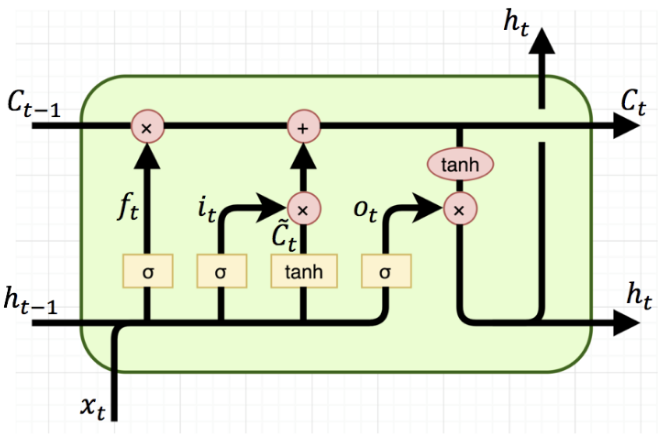
\includegraphics[width=.75\linewidth]{images/lstm_arch.png}
  \caption{Архитектура блока LSTM. $f_t,\ i_t,\ o_t$ - вентили забывания, входа и выхода. $x_t$ -- входной сигнал, $h_t$ -- выходной сигнал и внутреннее состояние блока. $C_t,\ C_{t-1}$ -- состояния ячейки памяти на $t$-м и $t-1$-м шагах соответственно}
  \label{fig:lstm_arch}
\end{figure}


В случае использования сети долгой краткосрочной памяти $L$ векторов будут последовательно поданы на вход модели, начиная с  $\bar{x}_{i-L+1}$ и заканчивая $\bar{x}_{i}$, а на выходе модель будет выдавать прогноз $\hat{y}_{i+1}$. При обучении модель будет пытаться обеспечить на последнем слое такой вывод $\hat{y}_{i+1}$, который был бы максимально похож на прогнозируемое значение $\bar{y}_{i+1}$.

При решении задачи классификации для оценки результатов была использована такая метрика как площадь под ROC-кривой (Area Under Curve, ROC AUC). Главным преимуществом этой метрики является её инвариантность относительно баланса классов. Так, например, при балансе классов 1:9 (на 1 объект из ''положительного'' класса приходится 9 объектов из ''отрицательного класса'') метрика "точность", представляющая из себя долю правильно классифицированных примеров, будет нерепрезентативной: можно получить точность равную 90\% просто предсказывая для всех классов метку ''отрицательный''. При этом, правильно предсказанные 80\% объектов из положительного класса и 80\% правильных предсказаний для негативного класса выглядят как более желаемый результат, но позволяют достичь лишь точности в 80\%.

Поскольку, как известно, в задаче классификации предсказания модели лежат в интервале $[0, 1]$, принадлежность объекта к положительному или отрицательному классу ($y' \in \{1, -1\}$) зависят от коэффициента принадлежности к положительному классу $p$, предсказанного моделью, и выбранного порога $\omega_0$:
$$
y' =    \begin{cases}
			1, & p >= \omega_0\\
            -1, & p < \omega_0
	    \end{cases}
$$

Для вычисления метрики ROC AUC необходимо ввести понятия доли ложных положительных классификаций (False Positive Rate, FPR) и доли верных положительных классификаций (True Positive Rate, TPR):

$$
FPR(y,y') = \frac{\sum_{i=1}^N [y'_i = +1][y_i = -1]}{\sum_{i=1}^N [y_i = -1]}
$$

$$
TPR(y,y') = \frac{\sum_{i=1}^N [y'_i = +1][y_i = +1]}{\sum_{i=1}^N [y_i = +1]}.
$$

Видно, что значения FPR и TPR зависят от выбранного порога $\omega_0$. ROC-кривая показывает зависимость TPR от FPR при варьировании этого порога. Из ее свойств стоит отметить, что она проходит из точки (0, 0) при $\omega_0 = min_{i=1..N} p_i$ в точку (1, 1) при $\omega_0 = max_{i=1..N} p_i$. Площадь под этой кривой (AUC) представляет из себя агрегированную характеристику качества классификации, и чем больше значение этой площади, тем лучше модель.

В задаче регрессии было решено использовать метрику средней абсолютной нормированной ошибки (Mean absolute scaled error, MASE). Сама метрика представляет из себя значение средней абсолютной ошибки нормированное на величину изменчивости прогнозируемых значений и часто используется при оценке качества прогнозирования временных рядов.

Стоит отметить следующие свойства этой метрики:
\begin{itemize}
    \item Инвариантность к мастштабу значений: поскольку в рамках вычисления метрики производится нормировка на изменчивость прогнозируемых данных, эта метрика может быть использована для сравнения на данных разной величины.
    \item Адекватное поведение при $y \rightarrow 0$: многие другие метрики предполагают деление на истинные значения $y_i$ и таким образом принимают сильно смещенные значения при $y_i \rightarrow 0$. Это особенно заметно при вычислении метрик для таких задач, как прогнозирование температуры, где прогнозируемые значения могут быть разных знаков или часто быть равными 0.
     \item Симметричность: метрика средней абсолютной нормированной ошибки ''штрафует'' одинаково ошибки прогноза как в меньшую, так и в большую сторону.
\end{itemize}

Значение метрики вычисляется по следующей формуле:
$$
MASE(y, y') = \frac{MAE(y, y')}{\frac{1}{N-1}\sum_{i=2}^{N} |y_i - y_{i-1}|},
$$ где 
$$MAE(y, y') = \frac{1}{N}\sum_{i=1}^{N} |y_i - y'_i|$$
Здесь $y$ обозначает истинные метки для периода, а $y'$ - метки, предсказанные моделью.

\begin{figure}[t]
  \centering
  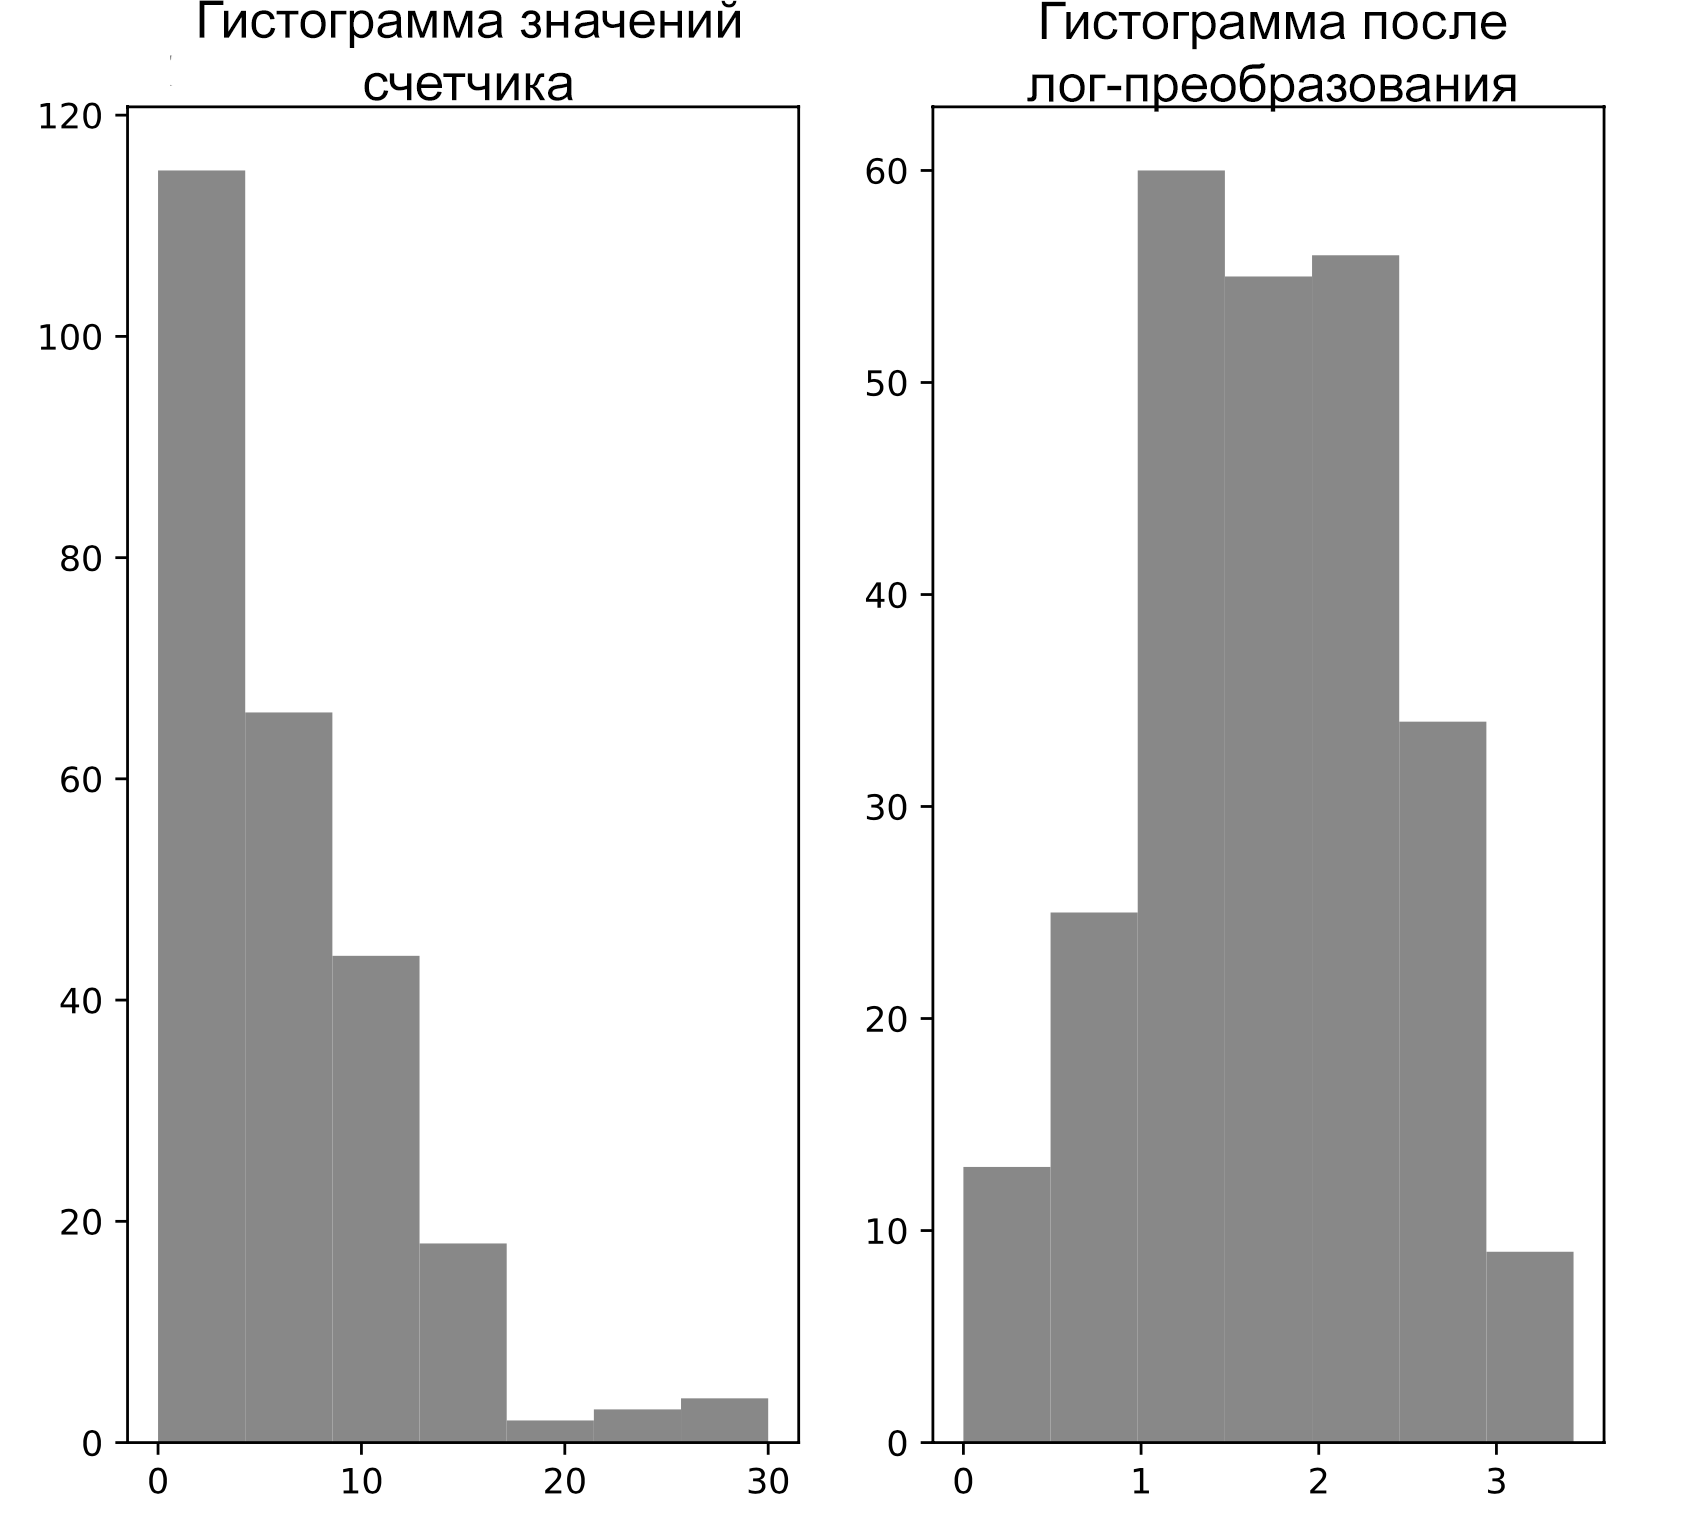
\includegraphics[width=0.45\linewidth]{images/log_hist}
  \caption{Логарифмическое преобразование значений счетчика}
  \label{fig:log_hist}
\end{figure}

По своей природе, целевая переменная в задаче регрессии является счетчиком событий. Исследовав распределение целевой переменной было выяснено, что она имеет распределение Пуассона \cite{pois_handbook}. Исходя из этого было решено предсказывать не количество $n$ событий, а величину $n' = log(1+n)$, восстанавливая затем $n$. Основная мотивация заключается в предположении, что логарифм величины распределенной по закону Пуассона моделировать легче как простыми моделями, такими как линейная регрессия, так и более сложными методами машинного обучения. В таком случае линейная модель регрессии будет называться "Пуассоновской регрессией".

В терминах решаемой задачи, обозначим истинное (прогнозируемое) значение целевой переменной как $y$, а прогноз модели, представляющий из себя логарифм счетчика, как $y'$.

Поскольку оценка моделью значения $y'$ представляет из себя $\mu = \mathbb{E}[\log(y+1)]$, корректное восстановление значения оригинальной целевой переменной $\mathbb{E}[y]$ можно произвести следующим образом: \cite{lognormal}:
$$\mathbb{E}[y]=e^{{\mu + \frac{\sigma ^{2}}{2}}} - 1,$$
где $\sigma$ это стандартное отклонение $y'$. Оценить значение $\sigma$ можно как среднеквадратичную ошибку, посчитанную на отложенной выборке.

Пример значений целевой переменной до и после применения логарифмического преобразования изображен на Рис. \ref{fig:log_hist}

 % Исследование и построение решения задачи

\subsection{Экспериментальная часть}
Для экспериментальной оценки реализации предложенного решения мы использовали набор данных GTD\_0616 \cite{db:gtd}.
% GTD description
Этот набор данных обладает следующими особенностями:
	\begin{enumerate}
		\item Содержит подробную информацию о терактах начиная с 1975 года
		\item Содержит 55'600 записей с 1991 по 2012 год
        \item Информация включает в себя подробное описание теракта: дата, страна, группировка, ущерб, ...
        \item Содержит разнородные признаки: количественные, категориальные и, для некоторых событий, текстовые описания.
	\end{enumerate}

% Data aggregation using NMF model
\subsubsection{Построение представления событий и интерпретируемость}
Чтобы получить необходимое нам представление событий в пространстве тематик, были использованы алгоритм матричной факторизации NMF и нейросетевой подход, основанный на автокодировщиках.
После преобразований, описанных в начале раздела \ref{subsub:repr} и агрегирования мы перешли от отдельных событий к \textit{временному периоду}, содержащему некоторые события с помощью усреднения значений тематик для событий, входящих в этот период. Далее будем называть этот период \textit{агрегационным периодом} или просто \textit{периодом}. Затем к предобработанным данным мы применяли методы построения представления событий, пример 10 выделенных тематик как результат работы алгоритма неотрицательной факторизации матриц можно видеть на  Рис. \ref{fig:features_example}.

\begin{figure}
  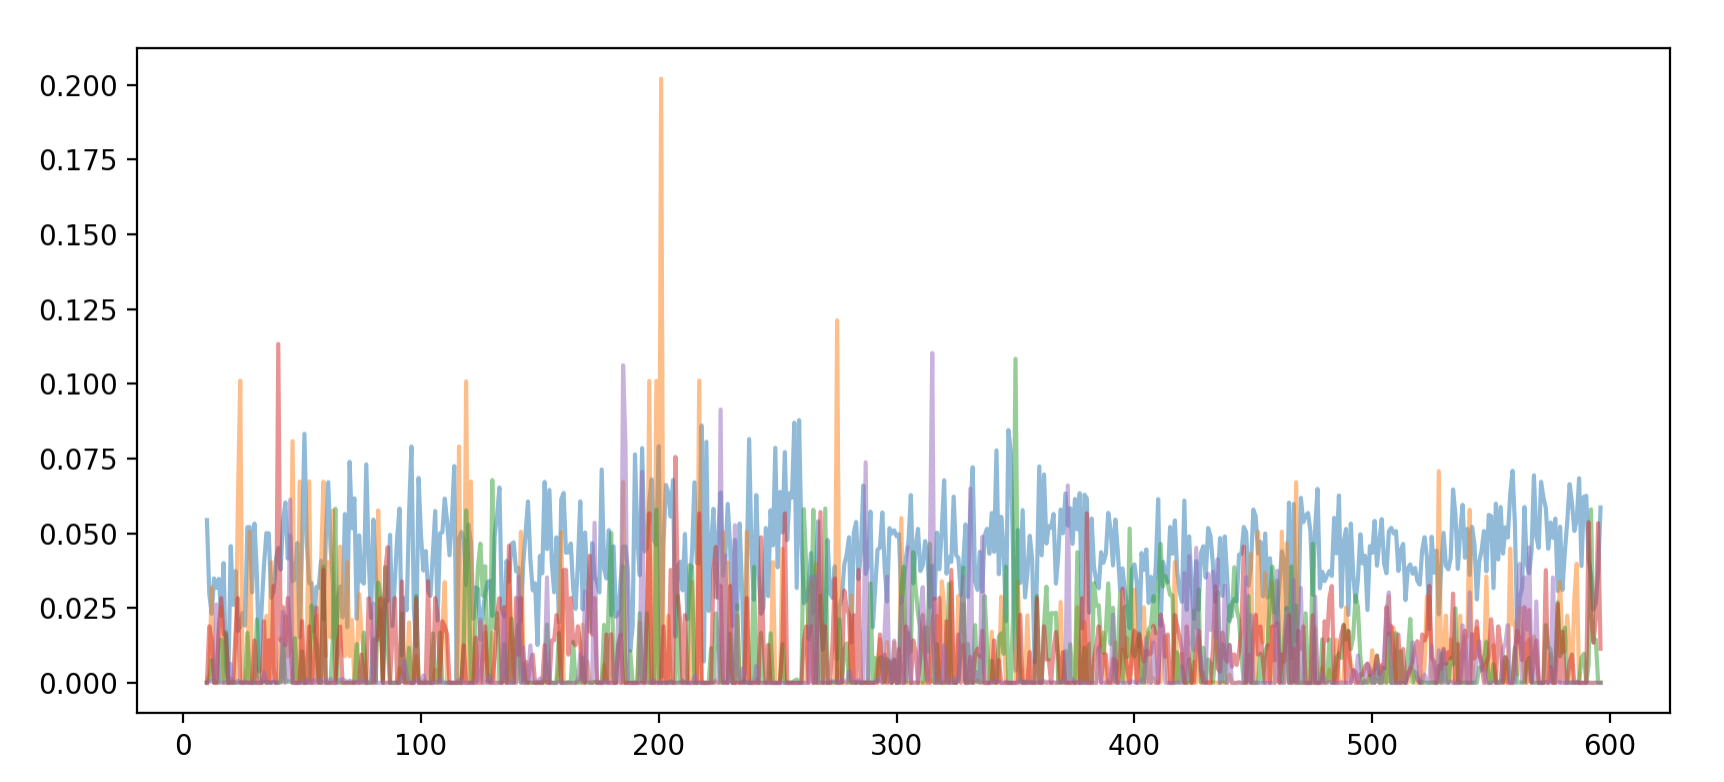
\includegraphics[width=\linewidth]{features_example.png}
  \caption{Пример временных рядов для тематик NMF}
  \label{fig:features_example}
\end{figure}

В случае с нейросетевым автокодировщиком, использовалась архитектура, описанная в таблице \ref{table:ae_arch}. Для кодировщика последовательно использовались полносвязные слои размерностей 256, 128 и 50 (размерность кода). Для декодировщика использовались полносвязные слои тех же размерностей, но в обратном порядке. Размерность входного вектора была равна 414, в рамках экспериментов были исследованы размерности скрытого кода равные 10 и 50. Для обучения модели применялась функция потерь $MAE$, описанная выше.
Количество эпох (т.е. количество проходов по всем имеющимся данным) при обучение модели было выбрано равным 100, начальный темп обучения был выбран равным  $2\cdot 10^{-3}$, также было использование экспоненциальное затухание темпа обучения: после каждой эпохи величина темпа обучения умножалась на 0.96.

\begin{table}
\centering
 \begin{tabular}{| c | c | c | c |} 
 \hline
 Название слоя & Тип слоя & Размер входа & Размер выхода \\
 \hline
 \hline
 кодировщик(1) & Полносвязный & 414 & 256 \\ 
 \hline
 кодировщик(2) & Полносвязный & 256 & 128 \\ 
 \hline
 кодировщик(3) & Полносвязный & 128 & 50 \\ 
 \hline
 декодировщик(1) & Полносвязный & 50 & 128 \\ 
 \hline
 декодировщик(2) & Полносвязный & 128 & 256 \\ 
 \hline
 декодировщик(3) & Полносвязный & 256 & 414 \\ 
 \hline
\end{tabular}
\caption{Архитектура автокодировщика}
\label{table:ae_arch}
\end{table}

Для интерпретации тематик методом, описанным в \ref{subsub:interp}, из набора данных были извлечены 19335 событий с текстовыми описаниями. После предобработки описаний и выделения слов был получен словарь размера 2311. После применения всей процедуры, описанной в \ref{subsub:interp} были получены наборы ключевых слов, описывающие тематики. Примеры таких ключевых слов для первых 5 тематик указаны в таблице \ref{table:kw_example}.

\begin{table}
\centering
 \begin{tabular}{c c} 
 \hline
 Тематика & Ключевые слова\\ 
 \hline
 \hline
 0 & used, sources, available, majority, listed, database, ...\\
 \hline
 1 & shot, civilian, distributed, bomb, detonated, ...\\
 \hline
 2 & taliban, shrine, perpetrators, tamil, rebels, group, ...\\
 \hline
 3 & released, hostage, kidnapping, status, abduction, ...\\
 \hline
 4 & indicated, military, police, civilian, detonating, ...\\
 \hline
 \end{tabular}
\caption{Примеры ключевых слов из описаний тематик }
\label{table:kw_example}
\end{table}


\subsubsection{Описание процесса обучения и тестирования} \label{train_process}
% NMF topics with lags as features
Метод прогнозирования, описываемый в моей работе, основывается на предположении, что вероятность наступления события (или количество событий) зависит от предшествующих событий, а точнее от значений тематик в агрегационных периодах, предшествующих периоду, для которого мы предсказываем эту вероятность.
В качестве признаков использовались значения тематик из $L$ предшествующих периодов, и таким образом для $k$ тематик размерность итогового пространства признаков становилась равна $L \cdot k$.

% target generation
Чтобы сформировать \textit{целевую переменную} необходимо было сначала определить события, которые нас интересуют (далее - \textit{целевые события}), в этой работе такие события определены как теракты, произошедшие в Ираке с типом атаки "взрыв". Затем каждому событию ставилась в соответствие метка: 1, если это интересующее нас событие и 0 иначе. 

Поскольку данные имеют очевидную временную составляющую, то разбиение на \textit{тренировочную} и \textit{тестовую} выборку производилось строго последовательно: первые 70\% данных отводились для тренировочной выборки, а оставшиеся 30\% - для тестовой.

% Metrics: ROC AUC, MAE
Для оценки качества решения в задаче классификации использовалась метрика ROC AUC, как уже было сказано выше, одно из ее преимуществ заключается в том, что она инвариантна к несбалансированности классов (в отличие, например, от метрики "Точность"). Поскольку в задачах прогнозирования событий реальные данные редко бывают сбалансированы, применение этой метрики является более разумным выбором для отражения качества прогноза.

В задаче регрессии для оценки решения была выбрана метрика MASE, которая рассчитывается по формуле, описанной в \ref{sect:event_forecast}.

% \subsection{Выбор разбиения данных} 
% \textit{Разбиение данных} - набор величин (год начала, год конца, длина периода агрегации, размер тренировочной выборки и правила для выбора целевых событий), характеризующий данные, получаемые после агрегации и генерации целевой переменной.\par
% % Automated time period choosing, different stats calculations
% Выше были определены признаки, которые будут использоваться для решения поставленных задач, и была упомянута проблема несбалансированных данных.
% На самом деле, если взять произвольные правила для определения целевого события (напр: страна Пакистан, тип атаки: Похищение) может оказаться, что ни один агрегационный период не содержит таких событий. Решение таких задач относится к области "прогнозирование экстремально редких событий (extreme rare event prediction) и выходит за рамки этой работы. 
% Чтобы избежать подобного дисбаланса было решено перебрать некоторое количество параметров, характеризующих данные, таких как
% \begin{enumerate}
%     \item Начальный и конечный год: 1997-2004 и 2004-2008 соответственно. Данные до начального и после конечного года мы не используем.
%     \item Длина периода агрегации: 1-15 дней, чем меньше, тем меньше значения целевой переменной.
%     \item Размер тренировочной выборки: 70\%, 80\%
%     \item Правила для выбора целевых событий: различные сочетания стран (Ирак/Пакистан/...) и типов атаки (Взрыв/Вооруженное нападение/...)
% \end{enumerate}
% В итоге была сформирована таблица, показывающая более-менее сбалансированные разбиения данных.

% Чтобы разбиение попало в таблицу, оно должно удовлетворять некоторым правилам.
% Для задачи классификации введем следующие обозначения:
% $\alpha := 0.1$,
% $r := 0.3$,
% $N_{train} := 300$,
% Обозначим долю положительных меток тренировочной и тестовой выборки как $Tr_m$ и $Ts_m$ соответственно, а размер тренировочной выборки как $Tr_{size}$.
% Тогда правила для разбиения выглядят следующим образом:
% \begin{itemize}
%     \item $Tr_m, Ts_m \in (\alpha, 1-\alpha$ (чтобы избежать дисбаланса классов в данных в целом)
%     \item $\frac{Tr_m}{Tr_m + Ts_m} \in (r, 1-r)$ (чтобы избежать дисбаланса между тренировочной и тестовой выборкой)
%     \item $Tr_{size} > N_{train}$ (чтобы было достаточно данных для обучения)
% \end{itemize}
% Для задачи регрессии введем дополнительно $r_{max} := 3$ и определим правила разбиения следующим образом:
% \begin{itemize}
%     \item $Ts_m > 0$
%     \item $\frac{Tr_m}{Ts_m}\in(1/r_{max}, r_{max})$ (избегаем дисбаланса между тренировочной и тестовой выборкой)
%     \item $Tr_{size} > N_{train}$ (чтобы было достаточно данных для обучения)
% \end{itemize}

% \begin{figure}
%   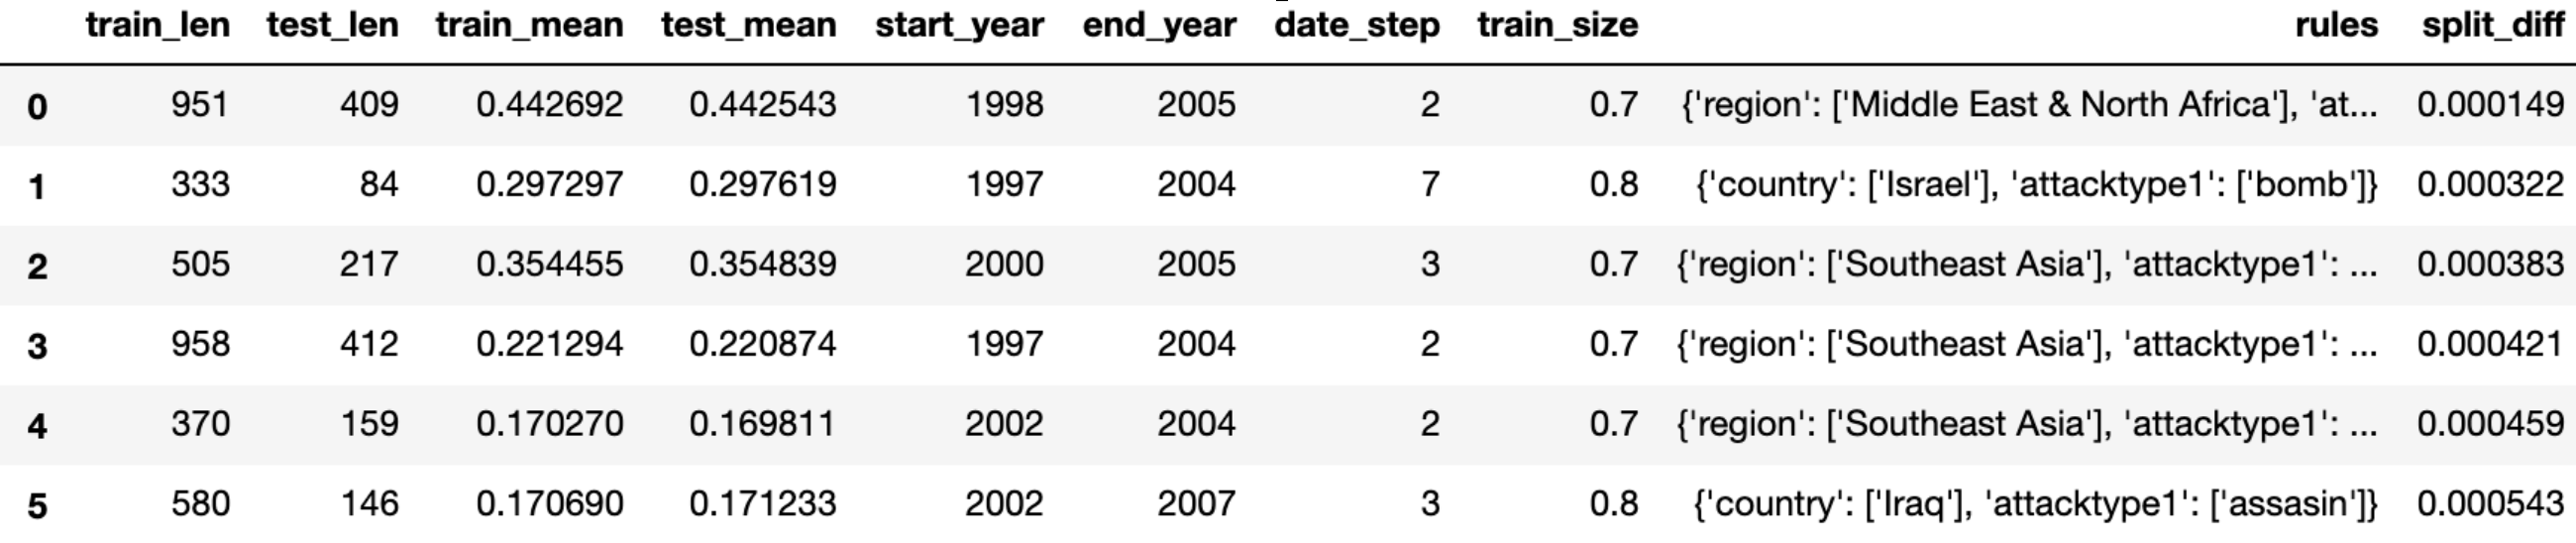
\includegraphics[width=\linewidth]{split_example.png}
%   \caption{Пример найденных разбиений для исходного набора данных}
%   \label{fig:split_example}
% \end{figure}

\subsubsection{Использование текстовых данных} \label{lda_topics}
% LDA model and document merging over agg period
В дополнение к существующим исходным признакам было решено использовать текстовые описания событий, а точнее соответствующие им вектора признаков, полученные с помощью модели Латентного размещения Дирихле (LDA) \cite{lda_orig}.
 
Модель Латентного размещения Дирихле представляет из себя статистическую модель, используемую в основном в задачах обработки текстов. Эта модель работает с документами, которые в свою очередь являются последовательностью термов (слов). Для заранее заданного числа скрытых (латентных) тем LDA позволяет построить два распределение: распределения тем по документам и распределения термов по темам. После того как модель обучена на $N$ документах для количества тем равного $K$ и количества различных термов равного $V$, мы получаем две матрицы весов $\theta \in \mathbf{R}^{N \times K}$ и $\phi \in \mathbf{R}^{K \times V}$, характеризующие параметры распределения Дирихле. Матрица $\theta$ отражает распределение тем по документам, а матрица $\phi$ -- распределение термов по темам.

Для получения значений скрытых тем новых документов необходимо их так же предобработать так же, как и тексты на которых производилось обучение, а затем, используя матрицу $\phi$ получить значения скрытых тем из текстового содержания документа.
После извлечения тематик каждому документу в соответствие ставится числовой вектор размерности $K$.

В рамках экспериментов алгоритм использования текстовых признаков с помощью модель Латентного размещения Дирихле выглядит следующим образом:
\begin{enumerate}
    \item Для каждого агрегационного периода получить единственный текстовый документ путем конкатенации (склеивания) всех текстовых описаний событий, входящих в период.
    \item Произвести классическую предобработку этих документов: удалить пунктуацию, нормализовать слов, удалить стоп-слова, ....
    \item Используя эти документы (точнее ту их часть, которая относится к тренировочной выборке) построить LDA-модель, т.е. построить распределение тематик по документам и распределение слов по тематикам для заданного количества тематик (в экспериментах количество тематик берется равным 10)
    \item Используя модель из предыдущего пункта получить 10 дополнительных признаков (соответствующих текстовым тематикам) для каждого агрегационного периода и использовать их вместе (с помощью конкатенации) с признаками, соответствующими скрытому представлению.
\end{enumerate}

Пример пяти тематик (их ключевых слов), выделенных с помощью LDA:
\begin{enumerate}
    \item incid bomb kill total relat
    \item claim respons group region kill
    \item group respons claim bomb injur
    \item incid target algerian take place
    \item algerian take place forc kill
\end{enumerate}

\begin{figure}
  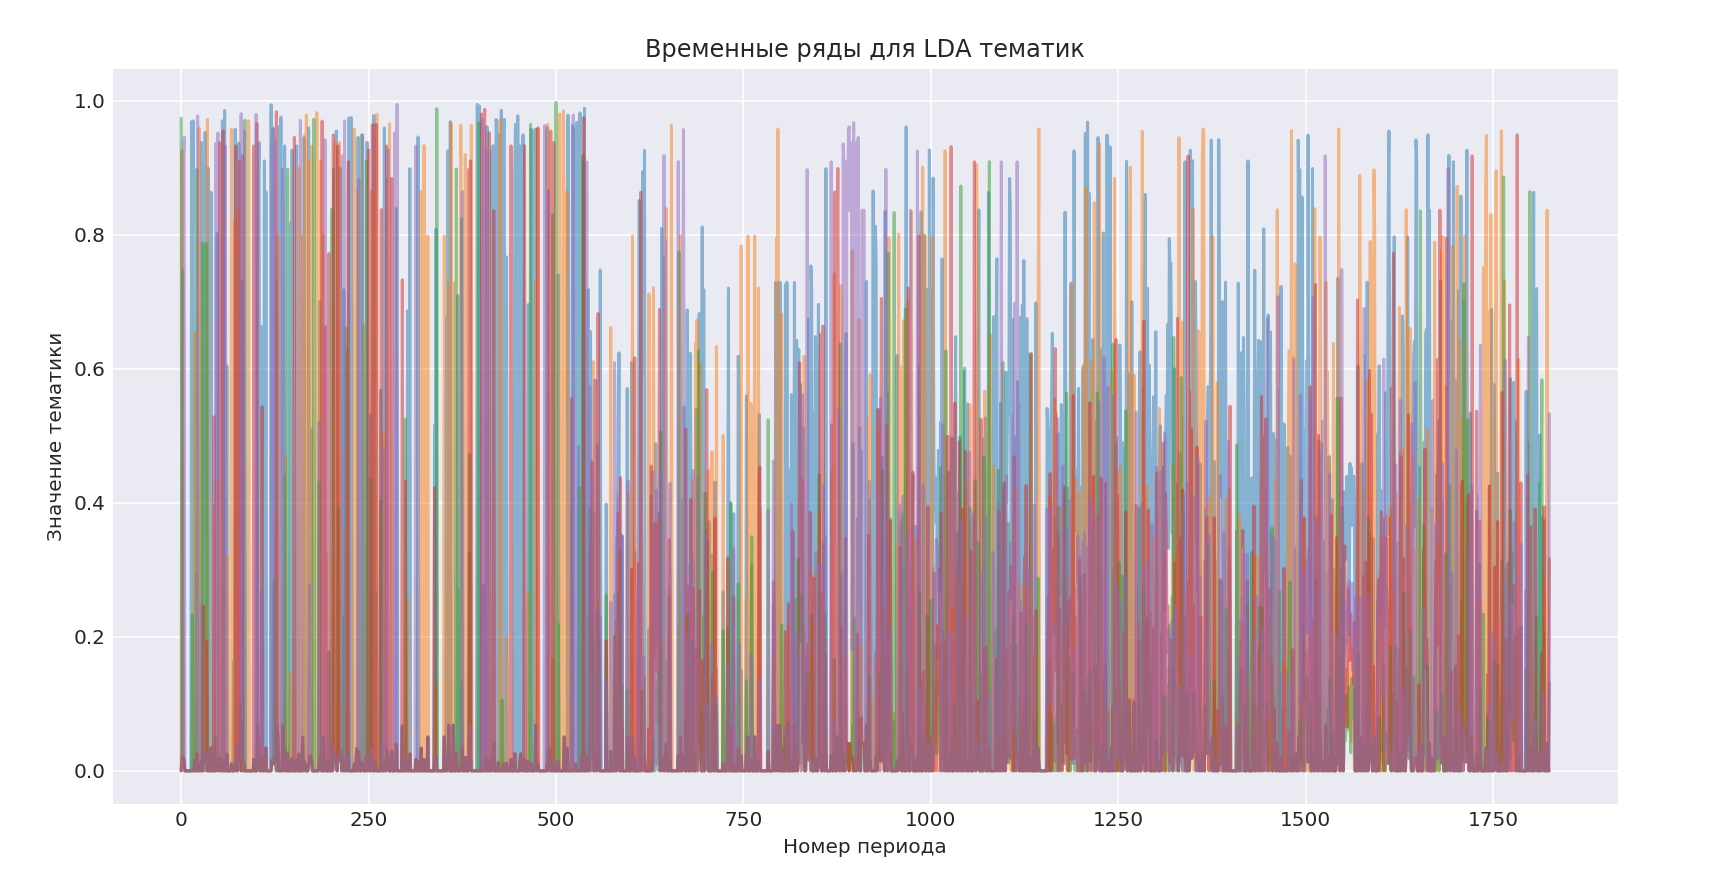
\includegraphics[width=\linewidth]{lda_example.png}
  \caption{Пример временных рядов для тематик LDA}
  \label{fig:lda_example}
\end{figure}

Пример соответствующих временных рядов можно увидеть на Рис. \ref{fig:lda_example}

\subsubsection{Результаты}
% Ниже приведены результаты для различных вариантов эксперимента.
Условия эксперимента:
\begin{enumerate}
    \item Год начала - 2002
    \item Год конца - 2008
    \item Длина агрегационного периода - 3 дня
    \item Тренировочная выборка: 70\%
    \item Целевые события: взрывы в Ираке (страна = Iraq, тип атаки = Bombing/Explosion)
\end{enumerate}
В рамках эксперимента были исследованы различные варианты представления событий -- с помощью NMF и с использованием автокодировщиков; количество тематик в экспериментах -- 10 и 50, так же вместе с тематиками были использованы дополнительные признаки AUX и REC.
В качестве моделей для прогнозирования были использованы классические модели классификации Logistic Regression (LogReg) и Random Forest Classifier (RFC), а так же нейронная сеть архитектуры LSTM.
Для задачи регрессии использовались модели Linear Regression (LinReg), Random Forest Regressor (RFR), а так же нейронная сеть архитектуры LSTM. Также варьировался размер окна исторических данных, которое мы принимали во внимание для построения прогноза. В текущем эксперименте были рассмотрены размеры окна равные 10 и 30.

В рамках экспериментов использовалась следующая архитектура сети LSTM: длина входной последовательности была равна 10 и 30 в зависимости от эксперимента и совпадала с размером окна исторических данных. Размерность скрытого слоя состояния LSTM-блока была равна размерности скрытого представления $k$ и принимала значения равные 10 и 50. При решении задачи прогнозирования вероятности события мы использовали функцию softmax для преобразования выхода сети в вероятности. В случае прогнозирования количества событий мы использовали линейную функцию активации. В процессе тренировки нейронной сети темп обучения был выбран равным $10^{-3}$, а количество эпох равным 50.

Обозначения:
\begin{itemize}
    \item  NMF\_N / AE\_N - использование тематик полученных с помощью NMF / Автокодировшика и с использованием N тематик
    \item + A - использование 2 дополнительных признаков (AUX), добавляющих авторегрессионную составляющую и описанных в \ref{train_process}
    \item + R - использование дополнительного признака, отвечающего за ошибку восстановления (реконструкции) в автокодировщике и описанного в \ref{train_process}
    %\item + text - использование 10 дополнительных тематик, описанных в \ref{lda_topics}
\end{itemize}

Перед изучением непосредственно результатов, важно отметить способ которым выбирались значения гиперпараметров для экспериментов. Пропорции разбиения данных на тренировочную и тестовую были выбраны как 70 к 30, поскольку это,  классический и наиболее часто используемый способ разбиения данных. Вторая причина выбора такого разбиения в том, что это позволяет оставить в тренировочном наборе достаточно данных для адекватного обучения модели и в то же время тестовый набор содержит в не слишком мало данных для валидации (тестирования). 

Длина агрегационного периода равная 3 дням была выбрана эмпирически, исходя из распределения целевой переменной. В общем случае длина интервала должна подбираться для каждой задачи отдельно, исходя из здравого смысла и поставленных целей. Так, например, если события редкие, то имеет смысл увеличить длину агрегационного периода. В случае если, например, стоит задача прогнозирования и изучения событий с недельной сезонностью, имеет смысл взять период агрегации равным 7 дням. 

Значения остальных гиперпараметров подбирались эмпирически. Поскольку основной целью данной работы является не получение максимальной точности на какой-то конкретной задаче, а описание и исследование применимости нового подхода к решению целого класса задач, тщательный перебор гиперпараметров не производился. Вероятнее всего, перебрав тщательным образом такие гиперпараметры как, например, число тематик и количество используемых исторических данных, можно значительно повысить итоговую точность прогнозирования.

\subsubsection{Прогнозирование вероятности события}
Поскольку задача прогнозирования вероятности события сводится к задаче классификации и определения, произойдет событие или нет, для решения этой задачи были выбраны модели классификации.
В таблицах \ref{table:clf-res-no-text} и \ref{table:clf-res-text} представлены результаты решения задачи по метрике ROC AUC (чем меньше, тем лучше) для различных моделей и условий тестирования. Лучшие из обученных моделей смогли достигнуть ROC AUC $\approx$ 0.75-0.79. Лучшие результаты получали модели прогнозирования LSTM для всех трех вариантов извлечения этих тематик (матричная факторизация, автокодировщик, автокодировщик + ошибка восстановления). Также можно увидеть, что вспомогательные признаки (AUX) помогли моделям достигать более качественных результатов. Что касается размера окна (кол-ва исторических данных, использовавшихся для прогнозирования), то в среднем модели LSTM достаточно хорошо работали для размеров окна равных 10 и 30, в то время как классические модели (Random Forest Classifier, Logistic Regression) показывали более хорошие результаты на меньшем размере окна. Это может быть связанно с тем, что количество признаков при увеличении размера окна росло линейно и моделям было сложнее найти нужные паттерны в данных.
При использовании текстовых описаний модели LSTM показали как результатов, причем независимо от метода построения представления событий. Модели логистической регрессии и случайного леса на некоторых методах представления событий показали выигрыш по качеству с добавлением текстовых описаний, а на других стали работать немного хуже. Это, опять же, можно объяснить меньшей гибкостью линейных моделей и модели случайного леса.

\begin{table}
\centering
\begin{tabular}{||p{3.8cm}|p{1.5cm}|p{1.5cm}|p{1.5cm}|p{1.5cm}|p{1.5cm}|p{1.5cm}||} 
\hline
& LSTM L=10 & LSTM L=30 & LogReg L=10 & LogReg L=30 & RFC L=10 & RFC L=30\\ \hline\hline
AE10 & 0.616 & 0.641 & 0.439 & 0.417 & 0.484 & 0.509\\ \hline
AE10+A & 0.747 & 0.749 & 0.654 & 0.578 & 0.583 & 0.598\\ \hline
AE50 & 0.651 & 0.655 & 0.567 & 0.574 & 0.656 & 0.637\\ \hline
AE50+A & 0.743 & 0.752 & 0.655 & 0.552 & 0.658 & 0.578\\ \hline
AE10+R & 0.696 & 0.656 & 0.480 & 0.608 & 0.509 & 0.566\\ \hline
AE10+AR & 0.764 & 0.744 & 0.653 & 0.572 & 0.609 & 0.615\\ \hline
AE50+R & 0.547 & 0.544 & 0.605 & 0.588 & 0.443 & 0.623\\ \hline
AE50+AR & 0.761 & 0.760 & 0.655 & 0.551 & 0.659 & 0.606\\ \hline
NMF10 & 0.618 & 0.605 & 0.577 & 0.526 & 0.637 & 0.606\\ \hline
NMF10+A & 0.746 & 0.746 & 0.653 & 0.561 & 0.701 & 0.670\\ \hline
NMF50 & 0.691 & 0.711 & 0.537 & 0.446 & 0.650 & 0.533\\ \hline
NMF50+A & 0.740 & \textbf{0.783} & 0.658 & 0.580 & 0.638 & 0.671\\ \hline
 \end{tabular}

\caption{\label{table:clf-res-text} Результаты по метрике ROC AUC для задачи классификации без использования текста}
\label{table:clf_res-no-text}
\end{table}


\begin{table}
\centering
\begin{tabular}{||p{3.8cm}|p{1.5cm}|p{1.5cm}|p{1.5cm}|p{1.5cm}|p{1.5cm}|p{1.5cm}||} 
\hline
& LSTM L=10 & LSTM L=30 & LogReg L=10 & LogReg L=30 & RFC L=10 & RFC L=30\\ \hline\hline
AE10 & 0.597 & 0.657 & 0.505 & 0.563 & 0.679 & 0.361\\ \hline
AE10+A & 0.764 & 0.747 & 0.642 & 0.599 & 0.673 & 0.665\\ \hline
AE50 & 0.655 & 0.678 & 0.523 & 0.550 & 0.624 & 0.631\\ \hline
AE50+A & 0.752 & 0.745 & 0.645 & 0.493 & 0.681 & 0.614\\ \hline
AE10+R & 0.608 & 0.628 & 0.523 & 0.564 & 0.424 & 0.474\\ \hline
AE10+AR & \textbf{0.795} & 0.758 & 0.642 & 0.576 & 0.644 & 0.619\\ \hline
AE50+R & 0.505 & 0.553 & 0.523 & 0.552 & 0.575 & 0.616\\ \hline
AE50+AR & 0.736 & 0.759 & 0.644 & 0.523 & 0.674 & 0.504\\ \hline
NMF10 & 0.612 & 0.743 & 0.476 & 0.563 & 0.652 & 0.615\\ \hline
NMF10+A & 0.601 & 0.753 & 0.644 & 0.544 & 0.674 & 0.567\\ \hline
NMF50 & 0.776 & 0.688 & 0.484 & 0.547 & 0.575 & 0.498\\ \hline
NMF50+A & 0.741 & 0.753 & 0.645 & 0.569 & 0.688 & 0.625\\ \hline
 \end{tabular}
\caption{\label{table:clf-res-no-text} Результаты по метрике ROC AUC для задачи классификации с использованием текста}
\label{table:clf_res-text}
\end{table}

\begin{figure}
  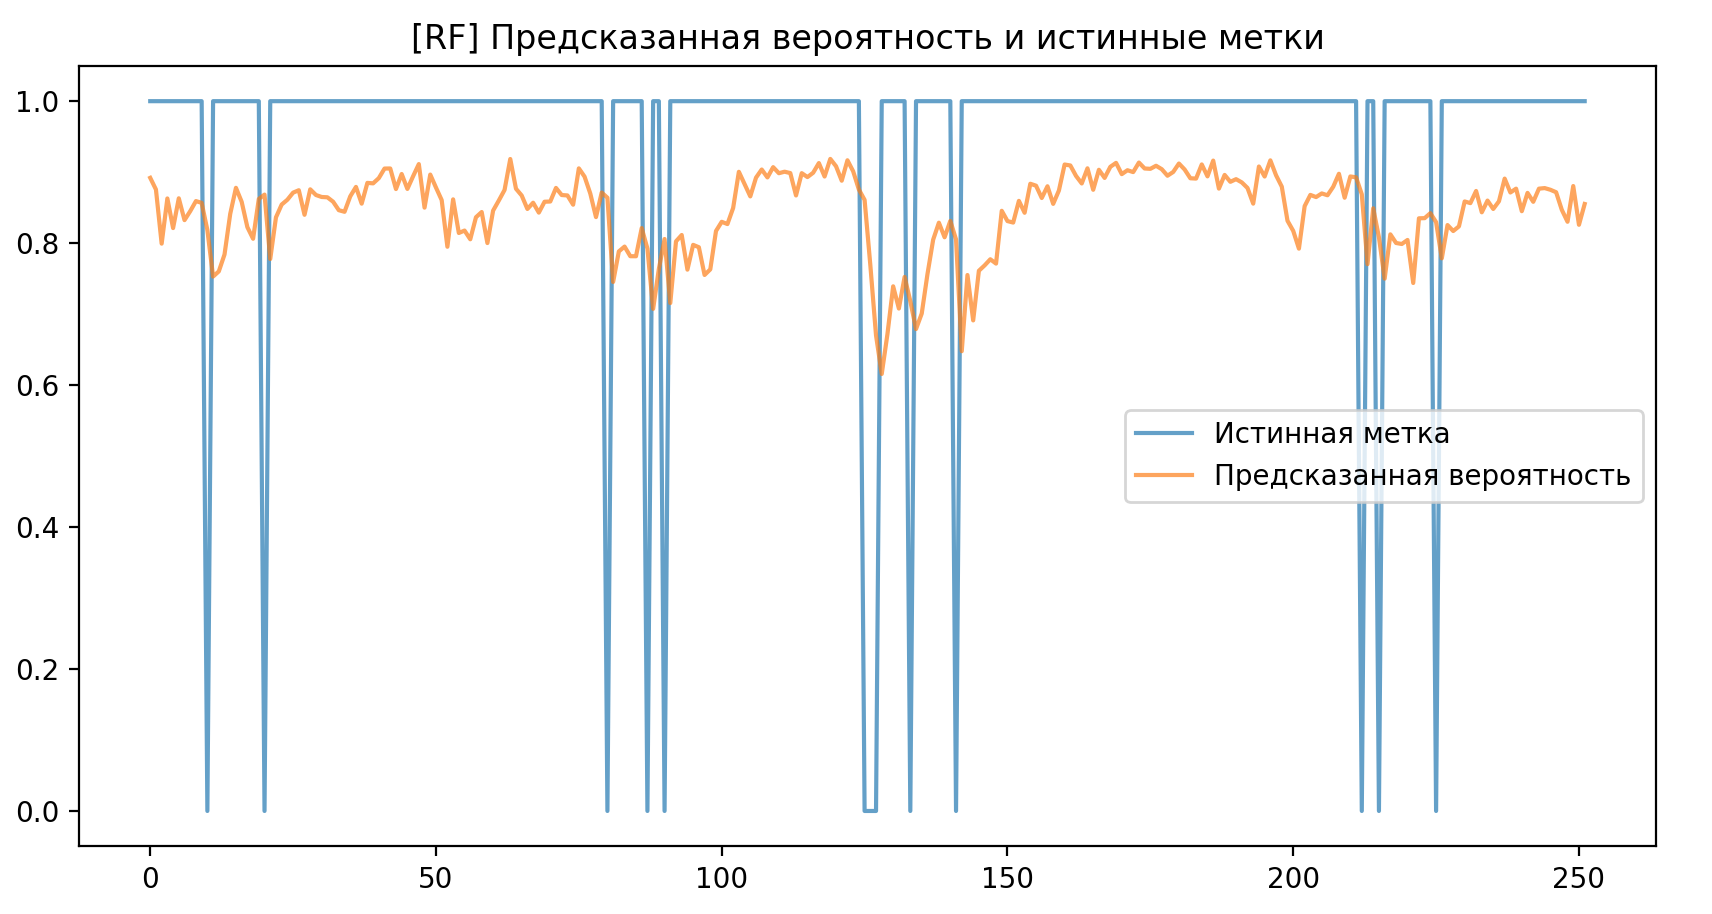
\includegraphics[width=\linewidth]{rf_clf_example.png}
  \caption{Пример работы модели классификации}
  \label{fig:rf_clf_example}
\end{figure}

\subsubsection{Прогнозирование количества событий}
Задача прогнозирования количества событий является задачей регрессии и может быть решена соответствующими моделями. В рамках экспериментов были рассмотрены модели линейной регрессии, случайного леса и нейросетевая модель архитектуры LSTM.
В таблицах \ref{table:reg-res-no-text}, \ref{table:reg-res} \ref{table:reg-res-no-text-log} и \ref{table:reg-res-log} представлены результаты решения задачи регрессии по метрике MASE (чем меньше, тем лучше) для различных моделей и условий тестирования.

Как было сказано в \ref{sect:event_forecast}, мы будем прогнозировать не целевую переменную, а ее логарифм. Поскольку для восстановления исходного значения целевой переменной требуется отложенная (валидационная) выборка для подсчета ошибки, разбиение данных в экспериментах будет производиться в пропорции 0.7 (тренировочная выборка) + 0.1 (валидационная) + 0.2 (тестовая). Таблицы \ref{table:reg-res-no-text} и \ref{table:reg-res} приведены для сравнения результатов с использованием и без использования логарифмического преобразования.

Лучшие из обученных моделей смогли достигнуть MASE $\approx$ 0.83-0.84. Лучшие результаты получали модели прогнозирования RFR, вспомогательные признаки (AUX) снова помогли моделям достигать более качественных результатов. Лучшим методом извлечения скрытых тематик оказался метод, основанный на автокодировщиках. В таблицах \ref{table:reg-res-no-text-log} и \ref{table:reg-res-log} видно, что значения метрики MASE для модели LinReg иногда становятся $\gg 1$. Это связанно с тем, что модель линейной регрессии показывает неудовлетворительные результаты на валидационной выборке. И, поскольку при восстановлении истинного значения целевой переменной используется среднеквадратичная ошибка по валидационной выборке, как описано в \ref{subsub:forecasting}, результаты модели оказываются сильно смещенными, вызывая аномально большие значения ошибки на тестовой выборке.

\begin{table}
\centering
\begin{tabular}{||p{3.8cm}|p{1.5cm}|p{1.5cm}|p{1.5cm}|p{1.5cm}|p{1.5cm}|p{1.5cm}||} 
\hline
& LSTM L=10 & LSTM L=30 & LinReg L=10 & LinReg L=30 & RFR L=10 & RFR L=30\\ \hline\hline
AE10 & 1.218 & 1.204 & 1.119 & 1.191 & 1.241 & 1.265\\ \hline
AE10+A & 1.050 & 1.050 & 0.909 & 1.074 & 0.890 & 0.909\\ \hline
AE10+R & 1.092 & 1.096 & 1.121 & 1.193 & 1.239 & 1.287\\ \hline
AE10+AR & 1.054 & 1.072 & 0.911 & 1.102 & 0.886 & 0.910\\ \hline
AE50 & 1.119 & 1.155 & 1.180 & 1.657 & 1.244 & 1.257\\ \hline
AE50+A & 1.084 & 1.055 & 1.632 & 1.616 & 0.883 & 0.904\\ \hline
AE50+R & 1.040 & 1.039 & 1.209 & 1.580 & 1.243 & 1.278\\ \hline
AE50+AR & 1.059 & 1.056 & 1.632 & 1.758 & \textbf{0.876} & 0.916\\ \hline
NMF10 & 1.218 & 1.194 & 1.096 & 1.422 & 1.094 & 1.182\\ \hline
NMF10+A & 1.056 & 1.069 & 0.895 & 1.177 & 0.894 & 0.929\\ \hline
NMF50 & 1.136 & 1.128 & 1.336 & 1.112 & 1.092 & 1.155\\ \hline
NMF50+A & 1.076 & 1.061 & 1.468 & 1.181 & 0.913 & 0.912\\ \hline
\end{tabular}
\caption{Результаты по метрике MASE для задачи регрессии без использования текста и без использования лог-преобразования}
\label{table:reg-res-no-text}
\end{table}

\begin{center}
\begin{table}
 \begin{tabular}{||p{3.8cm}|p{1.5cm}|p{1.5cm}|p{1.5cm}|p{1.5cm}|p{1.5cm}|p{1.5cm}||} 
\hline
& LSTM L=10 & LSTM L=30 & LinReg L=10 & LinReg L=30 & RFR L=10 & RFR L=30\\ \hline\hline
AE10 & 1.104 & 1.151 & 1.292 & 2.151 & 1.295 & 1.323\\ \hline
AE10+A & 1.084 & 1.058 & 1.025 & 1.924 & 0.898 & 0.925\\ \hline
AE10+R & 1.148 & 1.133 & 1.312 & 1.920 & 1.287 & 1.306\\ \hline
AE10+AR & 1.047 & 1.067 & 1.029 & 1.745 & 0.896 & 0.929\\ \hline
AE50 & 1.148 & 1.120 & 3.492 & 1.862 & 1.300 & 1.307\\ \hline
AE50+A & 1.046 & 1.068 & 3.082 & 1.810 & 0.899 & 0.918\\ \hline
AE50+R & 1.124 & 1.136 & 2.840 & 1.967 & 1.305 & 1.307\\ \hline
AE50+AR & 1.057 & 1.051 & 2.152 & 2.126 & 0.895 & 0.919\\ \hline
NMF10 & 1.171 & 1.068 & 1.241 & 2.921 & 1.171 & 1.187\\ \hline
NMF10+A & 1.077 & 1.059 & 0.973 & 2.280 & \textbf{0.894} & 0.933\\ \hline
NMF50 & 1.168 & 1.108 & 3.534 & 1.212 & 1.123 & 1.148\\ \hline
NMF50+A & 1.072 & 1.062 & 3.094 & 1.205 & 0.902 & 0.910\\ \hline
\textbf{0.910}\\ \hline
\end{tabular}
\caption{\label{table:reg-res} Результаты по метрике MASE для задачи регрессии c использованием текста и без лог-преобразования}
\end{table}
\end{center}


\begin{table}
\centering
\begin{tabular}{||p{3.8cm}|p{1.5cm}|p{1.5cm}|p{1.5cm}|p{1.5cm}|p{1.5cm}|p{1.5cm}||} 
\hline
& LSTM L=10 & LSTM L=30 & LinReg L=10 & LinReg L=30 & RFR L=10 & RFR L=30\\ \hline\hline
AE10 & 1.128 & 1.100 & 1.017 & 1.020 & 1.139 & 1.141\\ \hline
AE10+A & 1.054 & 1.014 & 1.028 & 1.729 & 0.848 & 0.875\\ \hline
AE50 & 1.059 & 1.035 & 1.127 & 3.075 & 1.073 & 1.105\\ \hline
AE50+A & 1.017 & 1.012 & 1.171 & 6.938 & 0.836 & 0.886\\ \hline
AE10+R & 1.105 & 1.068 & 1.046 & 1.087 & 1.135 & 1.151\\ \hline
AE10+R+A & 1.031 & 1.022 & 1.006 & 1.869 & \textbf{0.829} & 0.872\\ \hline
AE50+R & 1.052 & 0.979 & 1.141 & 5.021 & 1.107 & 1.116\\ \hline
AE50+R+A & 1.072 & 1.024 & 8.402 & 9.042 & 0.834 & 0.872\\ \hline
NMF10 & 1.055 & 1.088 & 1.108 & 1.263 & 1.010 & 1.047\\ \hline
NMF10+A & 1.025 & 1.032 & 1.008 & 1.582 & 0.862 & 0.898\\ \hline
NMF50 & 1.006 & 1.003 & 5.073 & 1.060 & 1.026 & 1.063\\ \hline
NMF50+A & 1.070 & 1.015 & 9.072 & 1.354 & 0.856 & 0.916\\ \hline
\end{tabular}
\caption{Результаты по метрике MASE для задачи регрессии c использованием лог-преобразования и без использования текста}
\label{table:reg-res-no-text-log}
\end{table}

\begin{center}
\begin{table}
 \begin{tabular}{||p{3.8cm}|p{1.5cm}|p{1.5cm}|p{1.5cm}|p{1.5cm}|p{1.5cm}|p{1.5cm}||} 
\hline
& LSTM L=10 & LSTM L=30 & LinReg L=10 & LinReg L=30 & RFR L=10 & RFR L=30\\ \hline\hline
AE10 & 1.057 & 1.051 & 1.216 & 5.461 & 1.149 & 1.172\\ \hline
AE10+A & 1.044 & 1.021 & 1.071 & 2.431 & 0.850 & 0.875\\ \hline
AE50 & 1.069 & 1.030 & 1.429 & 1.835 & 1.098 & 1.101\\ \hline
AE50+A & 1.047 & 1.024 & 1.283 & 2.097 & 0.859 & 0.869\\ \hline
AE10+R & 1.087 & 1.050 & 1.260 & 2.983 & 1.156 & 1.173\\ \hline
AE10+R+A & 1.041 & 1.030 & 1.082 & 4.846 & \textbf{0.843} & 0.868\\ \hline
AE50+R & 1.058 & 1.048 & 3.185 & 2.193 & 1.083 & 1.106\\ \hline
AE50+R+A & 1.035 & 1.029 & 9.062 & 1.089 & \textbf{0.843} & 0.891\\ \hline
NMF10 & 1.085 & 1.121 & 1.283 & 2.061 & 1.015 & 1.075\\ \hline
NMF10+A & 1.036 & 1.006 & 1.098 & 6.303 & 0.844 & 0.927\\ \hline
NMF50 & 1.114 & 1.175 & 5.817 & 1.112 & 1.056 & 1.060\\ \hline
NMF50+A & 1.047 & 1.028 & 3.428 & 3.692 & 0.861 & 0.914\\ \hline
\end{tabular}
\caption{\label{table:reg-res-log} Результаты по метрике MASE для задачи регрессии c использованием лог-преобразования и с использованием текста}
\end{table}
\end{center}

\begin{figure}
  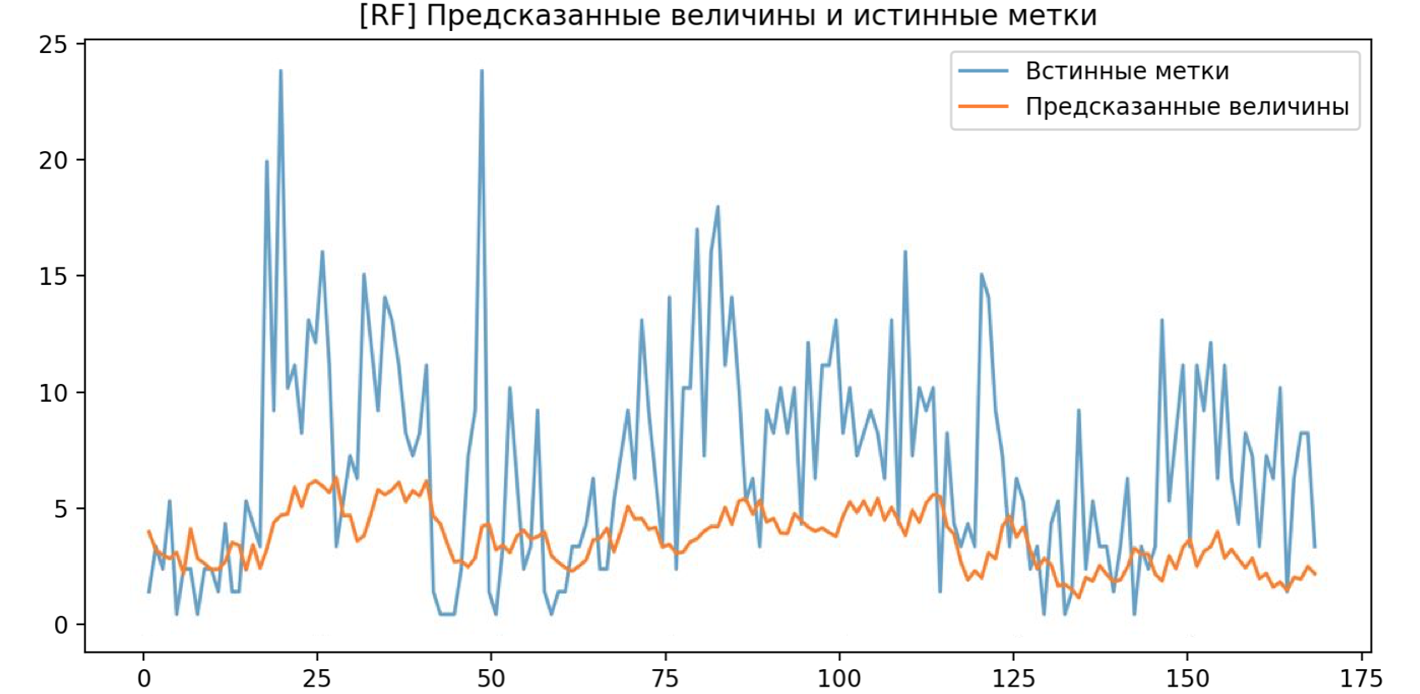
\includegraphics[width=\linewidth]{images/reg_noaux.png}
  \caption{Пример работы модели регрессии без использования AUX признаков}
  \label{fig:rf_reg_noaux}
\end{figure}

\begin{figure}
  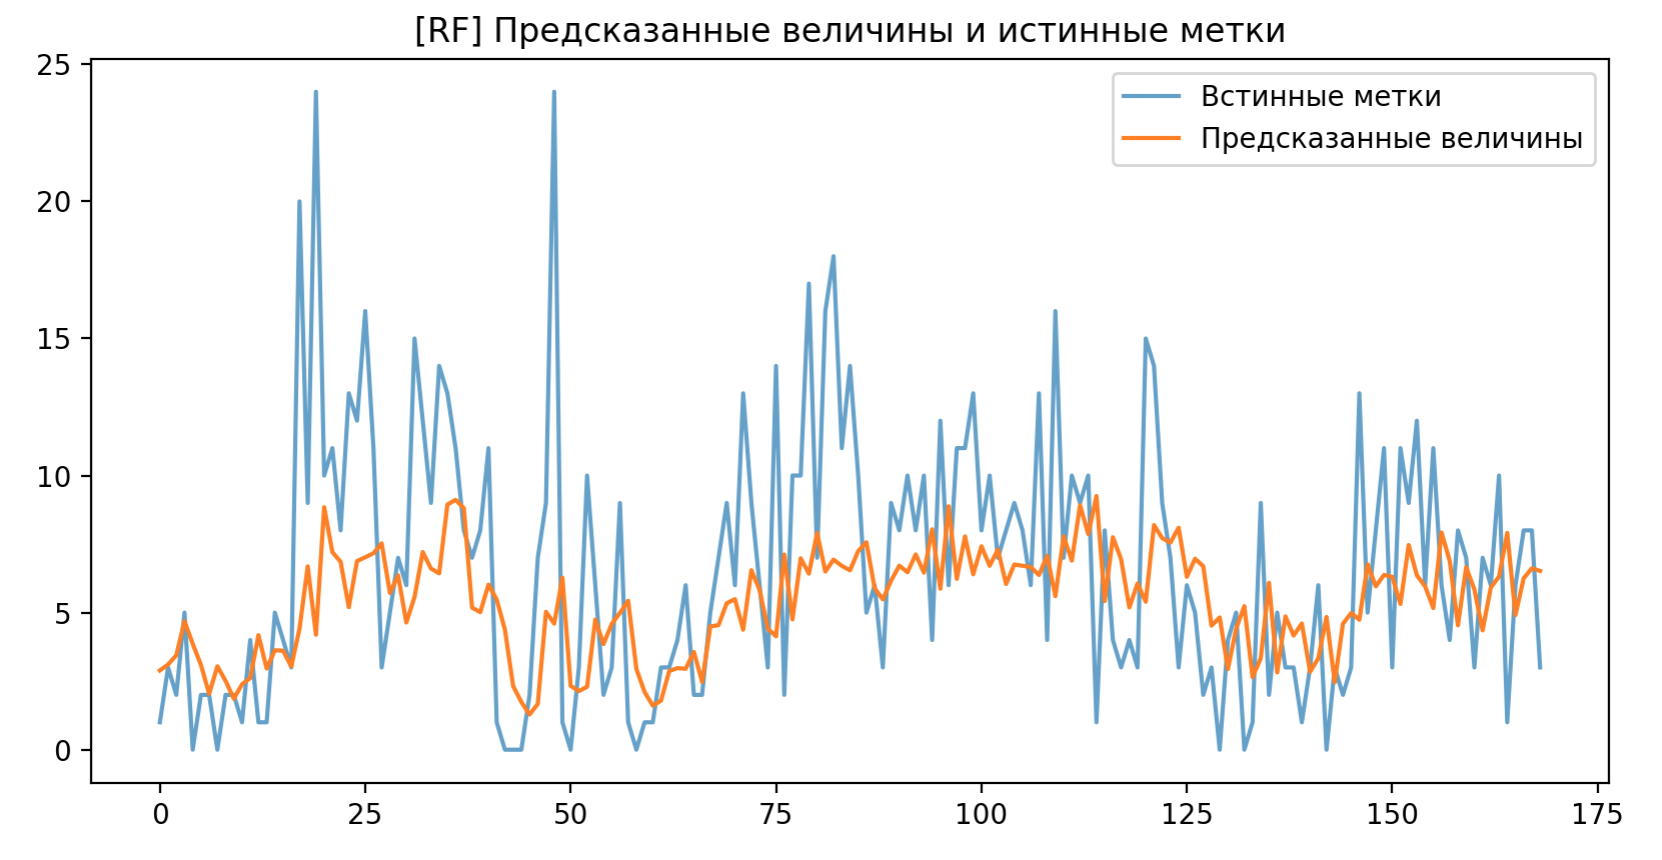
\includegraphics[width=\linewidth]{rf_reg_example.png}
  \caption{Пример работы модели регрессии с использованием AUX признаков}
  \label{fig:rf_reg_example}
\end{figure}


\subsubsection{Анализ полученных результатов}
В задаче классификации нейронные сети с LSTM-архитектурой оставляют остальные модели далеко позади, а добавление вспомогательных признаков 
(+A, +AR) позволяет улучшить качество прогноза на 10-40\%, в зависимости от типа модели. Это означает, что авторегрессионная компонента очень важна для точных прогнозов. Использование текста позволяет незначительно улучшить результаты (+1.5\%), но применимость текстовых признаков в целом зависит от типа модели. На Рис. \ref{fig:rf_reg_noaux} и \ref{fig:rf_reg_example} приведены примеры результатов работы модели регрессии без использования вспомогательных признаков и с их использованием соответственно.

Результаты в задаче регрессии схожи с результатами, описанными выше, но в задаче регрессии лучшей моделью оказался RandomForest Regressor, а не нейросеть LSTM. Как и в задаче классификации, вспомогательные признаки позволили значительно улучшить качество прогноза (до 30\%, в зависимости от типа модели).
В отличие от результатов задачи классификации, использование текста снижает точность прогноза на 1.5-2\%, это означает, что текстовая информация может быть полезна при решении одних задач и бесполезна или даже вредна при решении других задач.
Результаты регрессии с использованием логарифмического преобразования представлены в таблицах \ref{table:reg-res-no-text} и \ref{table:reg-res-log}. Использование такого преобразования позволило улучшить качество прогноза на 5-6\%.

\section{Заключение}
В данной работе рассматривались методы представления сложноструктурированных событий и прогнозирования их потоков. По результатам исследования были выявлены ограничения существующих методов решения задачи и предложен подход, позволяющий одновременно получать универсальное представление сложноструктурированных событий в виде временного ряда и производить их прогнозирование.
Ранее в работах со схожей тематикой не рассматривалось какое-либо автоматическое выделение признаков для дальнейшего прогнозирования. Подход, описанный в данной работе, объединяет автоматизацию выделения признаков, достаточно универсальных и поддающихся агрегации и интерпретации с построением модели прогнозирования событий по выделенным признакам.
Во время работы над построением представления сложноструктурированных событий был разработан дополнительный метод, позволяющий сопоставить ключевые слова автоматически выделенным тематикам, т.о. позволяющий строить описание события с помощью ключевых слов на основании значений тематик для данного события.
По итогам проведения экспериментов были найдены модели прогнозирования и способы построения представления сложноструктурированных событий, показывающие наилучшие результаты прогнозирования на тестовых данных.
Таким образом, главными итогами данной  работы являются следующие результаты:
\begin{enumerate}
    \item Предложено и реализовано представление данных из базы сложноструктурированных событий, основанное на методах понижения размерности и позволяющее работать со всеми типами признаков: текстовыми, числовыми, категориальными
    \item Признаки, полученные с использованием предложенного метода представления сложноструктурированных событий, могут быть использованы при решении задачи прогнозирования событий
    \item Разработан вспомогательный способ интерпретации скрытых признаков (тематик) через доступные текстовые описания событий, позволяющий интерпретировать даже поведение тех скрытых признаков, которые были получены сложными нелинейными преобразованиями исходных данных
    \item Проведены эксперименты и оценена работа различных моделей для решения задач прогнозирования как количества событий, так и вероятности наступления события

\end{enumerate}
%\section{Дальнейшая работа}
\label{sec:further_work} \index{further_work}
Дальнейшая работа над этой задачей включает в себя
\begin{enumerate}
    \item Обогащение текстовых описаний с использованием внешних источников
    \item Исследование возможных способов улучшения качества моделей классификации и регрессии
\end{enumerate} % Дальнейшая работа
%\include{Chapter7}
%\include{Chapter8} % Заключение%
%\include{Chapter9} % Приложение%
%\include{Chapter10} % Приложение%

\nocite{*}
\bibliographystyle{gost71u} % Для соответствия требованиям об оформлении списка литературы
\bibliography{references}

%\include{Appendix} % Приложение

\end{document}
